\documentclass[1p]{elsarticle_modified}
%\bibliographystyle{elsarticle-num}

%\usepackage[colorlinks]{hyperref}
%\usepackage{abbrmath_seonhwa} %\Abb, \Ascr, \Acal ,\Abf, \Afrak
\usepackage{amsfonts}
\usepackage{amssymb}
\usepackage{amsmath}
\usepackage{amsthm}
\usepackage{scalefnt}
\usepackage{amsbsy}
\usepackage{kotex}
\usepackage{caption}
\usepackage{subfig}
\usepackage{color}
\usepackage{graphicx}
\usepackage{xcolor} %% white, black, red, green, blue, cyan, magenta, yellow
\usepackage{float}
\usepackage{setspace}
\usepackage{hyperref}

\usepackage{tikz}
\usetikzlibrary{arrows}

\usepackage{multirow}
\usepackage{array} % fixed length table
\usepackage{hhline}

%%%%%%%%%%%%%%%%%%%%%
\makeatletter
\renewcommand*\env@matrix[1][\arraystretch]{%
	\edef\arraystretch{#1}%
	\hskip -\arraycolsep
	\let\@ifnextchar\new@ifnextchar
	\array{*\c@MaxMatrixCols c}}
\makeatother %https://tex.stackexchange.com/questions/14071/how-can-i-increase-the-line-spacing-in-a-matrix
%%%%%%%%%%%%%%%

\usepackage[normalem]{ulem}

\newcommand{\msout}[1]{\ifmmode\text{\sout{\ensuremath{#1}}}\else\sout{#1}\fi}
%SOURCE: \msout is \stkout macro in https://tex.stackexchange.com/questions/20609/strikeout-in-math-mode

\newcommand{\cancel}[1]{
	\ifmmode
	{\color{red}\msout{#1}}
	\else
	{\color{red}\sout{#1}}
	\fi
}

\newcommand{\add}[1]{
	{\color{blue}\uwave{#1}}
}

\newcommand{\replace}[2]{
	\ifmmode
	{\color{red}\msout{#1}}{\color{blue}\uwave{#2}}
	\else
	{\color{red}\sout{#1}}{\color{blue}\uwave{#2}}
	\fi
}

\newcommand{\Sol}{\mathcal{S}} %segment
\newcommand{\D}{D} %diagram
\newcommand{\A}{\mathcal{A}} %arc


%%%%%%%%%%%%%%%%%%%%%%%%%%%%%5 test

\def\sl{\operatorname{\textup{SL}}(2,\Cbb)}
\def\psl{\operatorname{\textup{PSL}}(2,\Cbb)}
\def\quan{\mkern 1mu \triangleright \mkern 1mu}

\theoremstyle{definition}
\newtheorem{thm}{Theorem}[section]
\newtheorem{prop}[thm]{Proposition}
\newtheorem{lem}[thm]{Lemma}
\newtheorem{ques}[thm]{Question}
\newtheorem{cor}[thm]{Corollary}
\newtheorem{defn}[thm]{Definition}
\newtheorem{exam}[thm]{Example}
\newtheorem{rmk}[thm]{Remark}
\newtheorem{alg}[thm]{Algorithm}

\newcommand{\I}{\sqrt{-1}}
\begin{document}

%\begin{frontmatter}
%
%\title{Boundary parabolic representations of knots up to 8 crossings}
%
%%% Group authors per affiliation:
%\author{Yunhi Cho} 
%\address{Department of Mathematics, University of Seoul, Seoul, Korea}
%\ead{yhcho@uos.ac.kr}
%
%
%\author{Seonhwa Kim} %\fnref{s_kim}}
%\address{Center for Geometry and Physics, Institute for Basic Science, Pohang, 37673, Korea}
%\ead{ryeona17@ibs.re.kr}
%
%\author{Hyuk Kim}
%\address{Department of Mathematical Sciences, Seoul National University, Seoul 08826, Korea}
%\ead{hyukkim@snu.ac.kr}
%
%\author{Seokbeom Yoon}
%\address{Department of Mathematical Sciences, Seoul National University, Seoul, 08826,  Korea}
%\ead{sbyoon15@snu.ac.kr}
%
%\begin{abstract}
%We find all boundary parabolic representation of knots up to 8 crossings.
%
%\end{abstract}
%\begin{keyword}
%    \MSC[2010] 57M25 
%\end{keyword}
%
%\end{frontmatter}

%\linenumbers
%\tableofcontents
%
\newcommand\colored[1]{\textcolor{white}{\rule[-0.35ex]{0.8em}{1.4ex}}\kern-0.8em\color{red} #1}%
%\newcommand\colored[1]{\textcolor{white}{ #1}\kern-2.17ex	\textcolor{white}{ #1}\kern-1.81ex	\textcolor{white}{ #1}\kern-2.15ex\color{red}#1	}

{\Large $\underline{12a_{0712}~(K12a_{0712})}$}

\setlength{\tabcolsep}{10pt}
\renewcommand{\arraystretch}{1.6}
\vspace{1cm}\begin{tabular}{m{100pt}>{\centering\arraybackslash}m{274pt}}
\multirow{5}{120pt}{
	\centering
	\includegraphics[width=112pt]{../../../GIT/diagram.site/Diagrams/png/1513_12a_0712.png}\\
\ \ \ A knot diagram\footnotemark}&
\allowdisplaybreaks
\textbf{Linearized knot diagam} \\
\cline{2-2}
 &
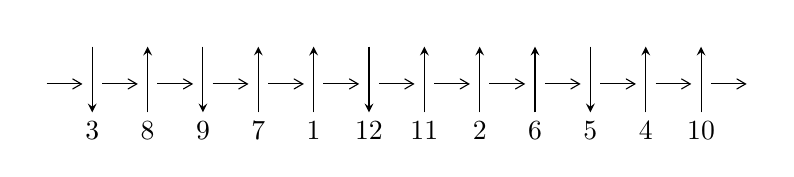
\begin{tikzpicture}[x=20pt, y=17pt]
	% nodes
	\node (C0) at (0, 0) {};
	\node (C1) at (1, 0) {};
	\node (C1U) at (1, +1) {};
	\node (C1D) at (1, -1) {3};

	\node (C2) at (2, 0) {};
	\node (C2U) at (2, +1) {};
	\node (C2D) at (2, -1) {8};

	\node (C3) at (3, 0) {};
	\node (C3U) at (3, +1) {};
	\node (C3D) at (3, -1) {9};

	\node (C4) at (4, 0) {};
	\node (C4U) at (4, +1) {};
	\node (C4D) at (4, -1) {7};

	\node (C5) at (5, 0) {};
	\node (C5U) at (5, +1) {};
	\node (C5D) at (5, -1) {1};

	\node (C6) at (6, 0) {};
	\node (C6U) at (6, +1) {};
	\node (C6D) at (6, -1) {12};

	\node (C7) at (7, 0) {};
	\node (C7U) at (7, +1) {};
	\node (C7D) at (7, -1) {11};

	\node (C8) at (8, 0) {};
	\node (C8U) at (8, +1) {};
	\node (C8D) at (8, -1) {2};

	\node (C9) at (9, 0) {};
	\node (C9U) at (9, +1) {};
	\node (C9D) at (9, -1) {6};

	\node (C10) at (10, 0) {};
	\node (C10U) at (10, +1) {};
	\node (C10D) at (10, -1) {5};

	\node (C11) at (11, 0) {};
	\node (C11U) at (11, +1) {};
	\node (C11D) at (11, -1) {4};

	\node (C12) at (12, 0) {};
	\node (C12U) at (12, +1) {};
	\node (C12D) at (12, -1) {10};
	\node (C13) at (13, 0) {};

	% arrows
	\draw[->,>={angle 60}]
	(C0) edge (C1) (C1) edge (C2) (C2) edge (C3) (C3) edge (C4) (C4) edge (C5) (C5) edge (C6) (C6) edge (C7) (C7) edge (C8) (C8) edge (C9) (C9) edge (C10) (C10) edge (C11) (C11) edge (C12) (C12) edge (C13) ;	\draw[->,>=stealth]
	(C1U) edge (C1D) (C2D) edge (C2U) (C3U) edge (C3D) (C4D) edge (C4U) (C5D) edge (C5U) (C6U) edge (C6D) (C7D) edge (C7U) (C8D) edge (C8U) (C9D) edge (C9U) (C10U) edge (C10D) (C11D) edge (C11U) (C12D) edge (C12U) ;
	\end{tikzpicture} \\
\hhline{~~} \\& 
\textbf{Solving Sequence} \\ \cline{2-2} 
 &
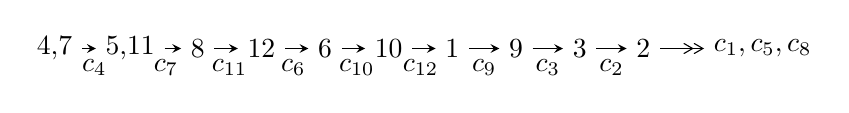
\begin{tikzpicture}[x=23pt, y=7pt]
	% node
	\node (A0) at (-1/8, 0) {4,7};
	\node (A1) at (17/16, 0) {5,11};
	\node (A2) at (17/8, 0) {8};
	\node (A3) at (25/8, 0) {12};
	\node (A4) at (33/8, 0) {6};
	\node (A5) at (41/8, 0) {10};
	\node (A6) at (49/8, 0) {1};
	\node (A7) at (57/8, 0) {9};
	\node (A8) at (65/8, 0) {3};
	\node (A9) at (73/8, 0) {2};
	\node (C1) at (1/2, -1) {$c_{4}$};
	\node (C2) at (13/8, -1) {$c_{7}$};
	\node (C3) at (21/8, -1) {$c_{11}$};
	\node (C4) at (29/8, -1) {$c_{6}$};
	\node (C5) at (37/8, -1) {$c_{10}$};
	\node (C6) at (45/8, -1) {$c_{12}$};
	\node (C7) at (53/8, -1) {$c_{9}$};
	\node (C8) at (61/8, -1) {$c_{3}$};
	\node (C9) at (69/8, -1) {$c_{2}$};
	\node (A10) at (11, 0) {$c_{1},c_{5},c_{8}$};

	% edge
	\draw[->,>=stealth]	
	(A0) edge (A1) (A1) edge (A2) (A2) edge (A3) (A3) edge (A4) (A4) edge (A5) (A5) edge (A6) (A6) edge (A7) (A7) edge (A8) (A8) edge (A9) ;
	\draw[->>,>={angle 60}]	
	(A9) edge (A10);
\end{tikzpicture} \\ 

\end{tabular} \\

\footnotetext{
The image of knot diagram is generated by the software ``\textbf{Draw programme}" developed by Andrew Bartholomew(\url{http://www.layer8.co.uk/maths/draw/index.htm\#Running-draw}), where we modified some parts for our purpose(\url{https://github.com/CATsTAILs/LinksPainter}).
}\phantom \\ \newline 
\centering \textbf{Ideals for irreducible components\footnotemark of $X_{\text{par}}$} 
 
\begin{align*}
I^u_{1}&=\langle 
1200 u^{27}-22896 u^{26}+\cdots+b-220937,\;-220937 u^{27}+3436077 u^{26}+\cdots+1003 a-276943727,\\
\phantom{I^u_{1}}&\phantom{= \langle  }u^{28}-21 u^{27}+\cdots-8019 u+1003\rangle \\
I^u_{2}&=\langle 
58 u^{21}-1336 u^{20}+\cdots+b-184389,\;-184389 u^{21}+4180402 u^{20}+\cdots+4223 a+427232464,\\
\phantom{I^u_{2}}&\phantom{= \langle  }u^{22}-24 u^{21}+\cdots-46453 u+4223\rangle \\
I^u_{3}&=\langle 
a^7 u+2 a^7-8 a^5 u-7 a^5-4 a^4 u- a^4+13 a^3 u+8 a^3+4 a^2 u-2 a^2-7 a u+b-3 a+3,\\
\phantom{I^u_{3}}&\phantom{= \langle  }a^8-3 a^6 u-5 a^6-3 a^5 u-2 a^5+6 a^4 u+7 a^4+5 a^3 u-3 a^2 u-4 a^2-2 a u+2 a+u+1,\;u^2+u+1\rangle \\
I^u_{4}&=\langle 
466047239 a^7 u^3+39554105 a^6 u^3+\cdots+1099016629 a+1191577537,\\
\phantom{I^u_{4}}&\phantom{= \langle  }5 a^6 u^3-6 a^5 u^3+\cdots+8 a+151,\;u^4+u^3-2 u+1\rangle \\
I^u_{5}&=\langle 
1.27748\times10^{33} u^{41}+1.90856\times10^{34} u^{40}+\cdots+6.44565\times10^{32} b-1.07355\times10^{33},\\
\phantom{I^u_{5}}&\phantom{= \langle  }1.07355\times10^{33} u^{41}+1.73807\times10^{34} u^{40}+\cdots+6.44565\times10^{32} a-5.56931\times10^{33},\;u^{42}+15 u^{41}+\cdots- u+1\rangle \\
I^u_{6}&=\langle 
32 a^7+2 a^6-9 a^5-140 a^4+168 a^3+111 a^2+61 b+49 a+13,\;a^8- a^6-4 a^5+6 a^4+6 a^3-5 a^2- a+2,\\
\phantom{I^u_{6}}&\phantom{= \langle  }u+1\rangle \\
I^u_{7}&=\langle 
1.76268\times10^{24} a^{11} u^{3}-8.39105\times10^{22} a^{10} u^{3}+\cdots+3.22438\times10^{23} a-1.26409\times10^{24},\\
\phantom{I^u_{7}}&\phantom{= \langle  }-4 a^{11} u^3+14 a^{10} u^3+\cdots-616 a-69,\;u^4+u^3-2 u+1\rangle \\
I^u_{8}&=\langle 
28032 a^{11} u+4413 a^{10} u+\cdots+275661 a-56296,\;- a^{11} u-5 a^{10} u+\cdots-2 a+1,\;u^2+u+1\rangle \\
I^u_{9}&=\langle 
31947 a^{11}+53734 b+\cdots+140465 a-40927,\\
\phantom{I^u_{9}}&\phantom{= \langle  }a^{12}+a^{11}- a^{10}+a^9+4 a^8+6 a^7-4 a^6-21 a^5+7 a^4+10 a^3-2 a^2-2 a+1,\;u+1\rangle \\
I^u_{10}&=\langle 
b-1,\;a+1,\;u+1\rangle \\
\\
I^v_{1}&=\langle 
a,\;b^4+b^2- b+1,\;v-1\rangle \\
I^v_{2}&=\langle 
a,\;b^6+b^5+2 b^4+2 b^3+2 b^2+2 b+1,\;v-1\rangle \\
\end{align*}
\raggedright * 12 irreducible components of $\dim_{\mathbb{C}}=0$, with total 243 representations.\\
\footnotetext{All coefficients of polynomials are rational numbers. But the coefficients are sometimes approximated in decimal forms when there is not enough margin.}
\newpage
\renewcommand{\arraystretch}{1}
\centering \section*{I. $I^u_{1}= \langle 1200 u^{27}-22896 u^{26}+\cdots+b-220937,\;-2.21\times10^{5} u^{27}+3.44\times10^{6} u^{26}+\cdots+1003 a-2.77\times10^{8},\;u^{28}-21 u^{27}+\cdots-8019 u+1003 \rangle$}
\flushleft \textbf{(i) Arc colorings}\\
\begin{tabular}{m{7pt} m{180pt} m{7pt} m{180pt} }
\flushright $a_{4}=$&$\begin{pmatrix}1\\0\end{pmatrix}$ \\
\flushright $a_{7}=$&$\begin{pmatrix}0\\u\end{pmatrix}$ \\
\flushright $a_{5}=$&$\begin{pmatrix}1\\- u^2\end{pmatrix}$ \\
\flushright $a_{11}=$&$\begin{pmatrix}220.276 u^{27}-3425.80 u^{26}+\cdots-1.85179\times10^{6} u+276115.\\-1200 u^{27}+22896 u^{26}+\cdots-2042510 u+220937\end{pmatrix}$ \\
\flushright $a_{8}=$&$\begin{pmatrix}0.500499 u^{27}-9.51047 u^{26}+\cdots+267.069 u-4.49751\\- u^{27}+20 u^{26}+\cdots-4008 u+502\end{pmatrix}$ \\
\flushright $a_{12}=$&$\begin{pmatrix}-979.724 u^{27}+19470.2 u^{26}+\cdots-3.89430\times10^{6} u+497052.\\-1200 u^{27}+22896 u^{26}+\cdots-2042510 u+220937\end{pmatrix}$ \\
\flushright $a_{6}=$&$\begin{pmatrix}-0.499501 u^{27}+9.48953 u^{26}+\cdots-233.931 u-3.49751\\- u^{26}+19 u^{25}+\cdots+3509 u-501\end{pmatrix}$ \\
\flushright $a_{10}=$&$\begin{pmatrix}1324.28 u^{27}-26401.8 u^{26}+\cdots+5.50756\times10^{6} u-706548.\\1022 u^{27}-17985 u^{26}+\cdots-2603150 u+429561\end{pmatrix}$ \\
\flushright $a_{1}=$&$\begin{pmatrix}428.276 u^{27}-10015.8 u^{26}+\cdots+6.01852\times10^{6} u-831197.\\2277 u^{27}-44386 u^{26}+\cdots+6582469 u-804129\end{pmatrix}$ \\
\flushright $a_{9}=$&$\begin{pmatrix}-1331.36 u^{27}+25723.6 u^{26}+\cdots-3.16627\times10^{6} u+372898.\\678 u^{27}-14540 u^{26}+\cdots+5772856 u-781700\end{pmatrix}$ \\
\flushright $a_{3}=$&$\begin{pmatrix}-14.3749 u^{27}+325.872 u^{26}+\cdots-186238. u+25702.1\\-48 u^{27}+972 u^{26}+\cdots-243822 u+31720\end{pmatrix}$ \\
\flushright $a_{2}=$&$\begin{pmatrix}-424.843 u^{27}+8504.71 u^{26}+\cdots-1.87799\times10^{6} u+241784.\\134 u^{27}-3113 u^{26}+\cdots+1909522 u-264635\end{pmatrix}$\\&\end{tabular}
\flushleft \textbf{(ii) Obstruction class $= -1$}\\~\\
\flushleft \textbf{(iii) Cusp Shapes $= 1298 u^{27}-23514 u^{26}+\cdots-1450392 u+283234$}\\~\\
\newpage\renewcommand{\arraystretch}{1}
\flushleft \textbf{(iv) u-Polynomials at the component}\newline \\
\begin{tabular}{m{50pt}|m{274pt}}
Crossings & \hspace{64pt}u-Polynomials at each crossing \\
\hline $$\begin{aligned}c_{1}\end{aligned}$$&$\begin{aligned}
&u^{28}+12 u^{27}+\cdots+160 u+64
\end{aligned}$\\
\hline $$\begin{aligned}c_{2},c_{8}\end{aligned}$$&$\begin{aligned}
&u^{28}+6 u^{27}+\cdots+40 u+8
\end{aligned}$\\
\hline $$\begin{aligned}c_{3}\end{aligned}$$&$\begin{aligned}
&u^{28}-6 u^{27}+\cdots-28744 u+3880
\end{aligned}$\\
\hline $$\begin{aligned}c_{4},c_{12}\end{aligned}$$&$\begin{aligned}
&u^{28}+21 u^{27}+\cdots+8019 u+1003
\end{aligned}$\\
\hline $$\begin{aligned}c_{5},c_{7},c_{9}\\c_{11}\end{aligned}$$&$\begin{aligned}
&u^{28}- u^{27}+\cdots- u+1
\end{aligned}$\\
\hline $$\begin{aligned}c_{6},c_{10}\end{aligned}$$&$\begin{aligned}
&u^{28}- u^{27}+\cdots-2 u+10
\end{aligned}$\\
\hline
\end{tabular}\\~\\
\newpage\renewcommand{\arraystretch}{1}
\flushleft \textbf{(v) Riley Polynomials at the component}\newline \\
\begin{tabular}{m{50pt}|m{274pt}}
Crossings & \hspace{64pt}Riley Polynomials at each crossing \\
\hline $$\begin{aligned}c_{1}\end{aligned}$$&$\begin{aligned}
&y^{28}+8 y^{27}+\cdots+58880 y+4096
\end{aligned}$\\
\hline $$\begin{aligned}c_{2},c_{8}\end{aligned}$$&$\begin{aligned}
&y^{28}+12 y^{27}+\cdots+160 y+64
\end{aligned}$\\
\hline $$\begin{aligned}c_{3}\end{aligned}$$&$\begin{aligned}
&y^{28}+4 y^{27}+\cdots-22855776 y+15054400
\end{aligned}$\\
\hline $$\begin{aligned}c_{4},c_{12}\end{aligned}$$&$\begin{aligned}
&y^{28}-21 y^{27}+\cdots+2369061 y+1006009
\end{aligned}$\\
\hline $$\begin{aligned}c_{5},c_{7},c_{9}\\c_{11}\end{aligned}$$&$\begin{aligned}
&y^{28}+9 y^{27}+\cdots+35 y+1
\end{aligned}$\\
\hline $$\begin{aligned}c_{6},c_{10}\end{aligned}$$&$\begin{aligned}
&y^{28}+19 y^{27}+\cdots+1736 y+100
\end{aligned}$\\
\hline
\end{tabular}\\~\\
\newpage\flushleft \textbf{(vi) Complex Volumes and Cusp Shapes}
$$\begin{array}{c|c|c}  
\text{Solutions to }I^u_{1}& \I (\text{vol} + \sqrt{-1}CS) & \text{Cusp shape}\\
 \hline 
\begin{aligned}
u &= \phantom{-}0.255884 + 0.893158 I \\
a &= -0.602738 - 0.627925 I \\
b &= -0.406606 + 0.699016 I\end{aligned}
 & -1.81341 - 7.68614 I & \phantom{-0.000000 -}0. + 8.22778 I \\ \hline\begin{aligned}
u &= \phantom{-}0.255884 - 0.893158 I \\
a &= -0.602738 + 0.627925 I \\
b &= -0.406606 - 0.699016 I\end{aligned}
 & -1.81341 + 7.68614 I & \phantom{-0.000000 } 0. - 8.22778 I \\ \hline\begin{aligned}
u &= \phantom{-}0.068858 + 0.795615 I \\
a &= \phantom{-}0.780549 + 0.451588 I \\
b &= \phantom{-}0.305543 - 0.652112 I\end{aligned}
 & \phantom{-}0.21428 - 2.63147 I & \phantom{-}2.98987 + 4.53509 I \\ \hline\begin{aligned}
u &= \phantom{-}0.068858 - 0.795615 I \\
a &= \phantom{-}0.780549 - 0.451588 I \\
b &= \phantom{-}0.305543 + 0.652112 I\end{aligned}
 & \phantom{-}0.21428 + 2.63147 I & \phantom{-}2.98987 - 4.53509 I \\ \hline\begin{aligned}
u &= \phantom{-}0.364425 + 0.513652 I \\
a &= -0.885699 - 1.065110 I \\
b &= -0.224323 + 0.843093 I\end{aligned}
 & -4.24210 - 0.23687 I & -3.97755 + 0.78715 I \\ \hline\begin{aligned}
u &= \phantom{-}0.364425 - 0.513652 I \\
a &= -0.885699 + 1.065110 I \\
b &= -0.224323 - 0.843093 I\end{aligned}
 & -4.24210 + 0.23687 I & -3.97755 - 0.78715 I \\ \hline\begin{aligned}
u &= -0.446227 + 0.363269 I \\
a &= \phantom{-}0.739248 - 0.644391 I \\
b &= \phantom{-}0.095785 - 0.556090 I\end{aligned}
 & \phantom{-}0.57015 - 1.33238 I & \phantom{-}4.21018 + 5.70611 I \\ \hline\begin{aligned}
u &= -0.446227 - 0.363269 I \\
a &= \phantom{-}0.739248 + 0.644391 I \\
b &= \phantom{-}0.095785 + 0.556090 I\end{aligned}
 & \phantom{-}0.57015 + 1.33238 I & \phantom{-}4.21018 - 5.70611 I \\ \hline\begin{aligned}
u &= \phantom{-}1.30381 + 0.63944 I \\
a &= \phantom{-}0.508862 + 0.586733 I \\
b &= -0.288283 - 1.090380 I\end{aligned}
 & -5.45715 + 1.59172 I & \phantom{-0.000000 } 0 \\ \hline\begin{aligned}
u &= \phantom{-}1.30381 - 0.63944 I \\
a &= \phantom{-}0.508862 - 0.586733 I \\
b &= -0.288283 + 1.090380 I\end{aligned}
 & -5.45715 - 1.59172 I & \phantom{-0.000000 } 0\\
 \hline 
 \end{array}$$\newpage$$\begin{array}{c|c|c}  
\text{Solutions to }I^u_{1}& \I (\text{vol} + \sqrt{-1}CS) & \text{Cusp shape}\\
 \hline 
\begin{aligned}
u &= \phantom{-}1.28320 + 0.83837 I \\
a &= \phantom{-}0.717468 + 0.432432 I \\
b &= -0.558117 - 1.156400 I\end{aligned}
 & -5.20632 + 10.84520 I & \phantom{-0.000000 } 0 \\ \hline\begin{aligned}
u &= \phantom{-}1.28320 - 0.83837 I \\
a &= \phantom{-}0.717468 - 0.432432 I \\
b &= -0.558117 + 1.156400 I\end{aligned}
 & -5.20632 - 10.84520 I & \phantom{-0.000000 } 0 \\ \hline\begin{aligned}
u &= \phantom{-}1.16856 + 1.02636 I \\
a &= -1.091200 - 0.031262 I \\
b &= \phantom{-}1.24305 + 1.15649 I\end{aligned}
 & \phantom{-}0.9229 + 21.6752 I & \phantom{-0.000000 } 0 \\ \hline\begin{aligned}
u &= \phantom{-}1.16856 - 1.02636 I \\
a &= -1.091200 + 0.031262 I \\
b &= \phantom{-}1.24305 - 1.15649 I\end{aligned}
 & \phantom{-}0.9229 - 21.6752 I & \phantom{-0.000000 } 0 \\ \hline\begin{aligned}
u &= \phantom{-}1.19278 + 1.00782 I \\
a &= -1.020190 - 0.114174 I \\
b &= \phantom{-}1.10179 + 1.16435 I\end{aligned}
 & -1.81840 + 13.23660 I & \phantom{-0.000000 } 0 \\ \hline\begin{aligned}
u &= \phantom{-}1.19278 - 1.00782 I \\
a &= -1.020190 + 0.114174 I \\
b &= \phantom{-}1.10179 - 1.16435 I\end{aligned}
 & -1.81840 - 13.23660 I & \phantom{-0.000000 } 0 \\ \hline\begin{aligned}
u &= \phantom{-}1.18001 + 1.03031 I \\
a &= \phantom{-}1.046090 + 0.029745 I \\
b &= -1.20375 - 1.11290 I\end{aligned}
 & \phantom{-}3.3671 + 16.3184 I & \phantom{-0.000000 } 0 \\ \hline\begin{aligned}
u &= \phantom{-}1.18001 - 1.03031 I \\
a &= \phantom{-}1.046090 - 0.029745 I \\
b &= -1.20375 + 1.11290 I\end{aligned}
 & \phantom{-}3.3671 - 16.3184 I & \phantom{-0.000000 } 0 \\ \hline\begin{aligned}
u &= \phantom{-}1.38335 + 0.78280 I \\
a &= -0.565439 - 0.415823 I \\
b &= \phantom{-}0.456694 + 1.017860 I\end{aligned}
 & -1.41308 + 6.14508 I & \phantom{-0.000000 } 0 \\ \hline\begin{aligned}
u &= \phantom{-}1.38335 - 0.78280 I \\
a &= -0.565439 + 0.415823 I \\
b &= \phantom{-}0.456694 - 1.017860 I\end{aligned}
 & -1.41308 - 6.14508 I & \phantom{-0.000000 } 0\\
 \hline 
 \end{array}$$\newpage$$\begin{array}{c|c|c}  
\text{Solutions to }I^u_{1}& \I (\text{vol} + \sqrt{-1}CS) & \text{Cusp shape}\\
 \hline 
\begin{aligned}
u &= \phantom{-}1.22841 + 1.05657 I \\
a &= \phantom{-}0.884436 + 0.007946 I \\
b &= -1.07806 - 0.94423 I\end{aligned}
 & \phantom{-}5.4565 + 13.1132 I & \phantom{-0.000000 } 0 \\ \hline\begin{aligned}
u &= \phantom{-}1.22841 - 1.05657 I \\
a &= \phantom{-}0.884436 - 0.007946 I \\
b &= -1.07806 + 0.94423 I\end{aligned}
 & \phantom{-}5.4565 - 13.1132 I & \phantom{-0.000000 } 0 \\ \hline\begin{aligned}
u &= \phantom{-}1.26956 + 1.06446 I \\
a &= -0.794082 - 0.027969 I \\
b &= \phantom{-}0.978364 + 0.880777 I\end{aligned}
 & \phantom{-}4.78086 + 7.54326 I & \phantom{-0.000000 } 0 \\ \hline\begin{aligned}
u &= \phantom{-}1.26956 - 1.06446 I \\
a &= -0.794082 + 0.027969 I \\
b &= \phantom{-}0.978364 - 0.880777 I\end{aligned}
 & \phantom{-}4.78086 - 7.54326 I & \phantom{-0.000000 } 0 \\ \hline\begin{aligned}
u &= -1.67808 + 0.17720 I \\
a &= \phantom{-}0.033642 - 0.204254 I \\
b &= \phantom{-}0.020260 - 0.348715 I\end{aligned}
 & \phantom{-}5.76082 - 2.91752 I & \phantom{-0.000000 } 0 \\ \hline\begin{aligned}
u &= -1.67808 - 0.17720 I \\
a &= \phantom{-}0.033642 + 0.204254 I \\
b &= \phantom{-}0.020260 + 0.348715 I\end{aligned}
 & \phantom{-}5.76082 + 2.91752 I & \phantom{-0.000000 } 0 \\ \hline\begin{aligned}
u &= \phantom{-}1.92546 + 0.15687 I \\
a &= -0.060515 - 0.375245 I \\
b &= \phantom{-}0.057653 + 0.732010 I\end{aligned}
 & \phantom{-}4.63509 + 3.17553 I & \phantom{-0.000000 } 0 \\ \hline\begin{aligned}
u &= \phantom{-}1.92546 - 0.15687 I \\
a &= -0.060515 + 0.375245 I \\
b &= \phantom{-}0.057653 - 0.732010 I\end{aligned}
 & \phantom{-}4.63509 - 3.17553 I & \phantom{-0.000000 } 0\\
 \hline 
 \end{array}$$\newpage\newpage\renewcommand{\arraystretch}{1}
\centering \section*{II. $I^u_{2}= \langle 58 u^{21}-1336 u^{20}+\cdots+b-184389,\;-1.84\times10^{5} u^{21}+4.18\times10^{6} u^{20}+\cdots+4223 a+4.27\times10^{8},\;u^{22}-24 u^{21}+\cdots-46453 u+4223 \rangle$}
\flushleft \textbf{(i) Arc colorings}\\
\begin{tabular}{m{7pt} m{180pt} m{7pt} m{180pt} }
\flushright $a_{4}=$&$\begin{pmatrix}1\\0\end{pmatrix}$ \\
\flushright $a_{7}=$&$\begin{pmatrix}0\\u\end{pmatrix}$ \\
\flushright $a_{5}=$&$\begin{pmatrix}1\\- u^2\end{pmatrix}$ \\
\flushright $a_{11}=$&$\begin{pmatrix}43.6630 u^{21}-989.913 u^{20}+\cdots+1.08626\times10^{6} u-101168\\-58 u^{21}+1336 u^{20}+\cdots-1927111 u+184389\end{pmatrix}$ \\
\flushright $a_{8}=$&$\begin{pmatrix}0.499882 u^{21}-10.9972 u^{20}+\cdots+20030.3 u-2105\\- u^{21}+22 u^{20}+\cdots-21115 u+2111\end{pmatrix}$ \\
\flushright $a_{12}=$&$\begin{pmatrix}-14.3370 u^{21}+346.087 u^{20}+\cdots-840852. u+83221\\-58 u^{21}+1336 u^{20}+\cdots-1927111 u+184389\end{pmatrix}$ \\
\flushright $a_{6}=$&$\begin{pmatrix}0.499882 u^{21}-11.9972 u^{20}+\cdots+22140.3 u-2106\\u^{21}-23 u^{20}+\cdots+23227 u-2112\end{pmatrix}$ \\
\flushright $a_{10}=$&$\begin{pmatrix}41.6630 u^{21}-970.913 u^{20}+\cdots+1.66903\times10^{6} u-161713\\2 u^{21}-22 u^{20}+\cdots-588420 u+61922\end{pmatrix}$ \\
\flushright $a_{1}=$&$\begin{pmatrix}72.6630 u^{21}-1625.91 u^{20}+\cdots+1.23544\times10^{6} u-108237\\-114 u^{21}+2650 u^{20}+\cdots-4438373 u+429323\end{pmatrix}$ \\
\flushright $a_{9}=$&$\begin{pmatrix}62.9946 u^{21}-1471.87 u^{20}+\cdots+2.59856\times10^{6} u-251727\\19 u^{21}-393 u^{20}+\cdots-557436 u+63322\end{pmatrix}$ \\
\flushright $a_{3}=$&$\begin{pmatrix}-10.1253 u^{21}+229.006 u^{20}+\cdots-152359. u+12682\\- u^{21}+13 u^{20}+\cdots+211150 u-21644\end{pmatrix}$ \\
\flushright $a_{2}=$&$\begin{pmatrix}0.468387 u^{21}-48.2413 u^{20}+\cdots+1.09162\times10^{6} u-112815\\34 u^{21}-771 u^{20}+\cdots+696795 u-61367\end{pmatrix}$\\&\end{tabular}
\flushleft \textbf{(ii) Obstruction class $= -1$}\\~\\
\flushleft \textbf{(iii) Cusp Shapes $= -166 u^{21}+3833 u^{20}-43763 u^{19}+327218 u^{18}-1793102 u^{17}+7643905 u^{16}-26278137 u^{15}+74562324 u^{14}-177325077 u^{13}+357053127 u^{12}-612487772 u^{11}+897797312 u^{10}-1124753307 u^9+1201124031 u^8-1087079978 u^7+825843900 u^6-518873251 u^5+263618515 u^4-104567593 u^3+30542893 u^2-5878416 u+563603$}\\~\\
\newpage\renewcommand{\arraystretch}{1}
\flushleft \textbf{(iv) u-Polynomials at the component}\newline \\
\begin{tabular}{m{50pt}|m{274pt}}
Crossings & \hspace{64pt}u-Polynomials at each crossing \\
\hline $$\begin{aligned}c_{1}\end{aligned}$$&$\begin{aligned}
&(u^{11}+5 u^{10}+\cdots+12 u-16)^{2}
\end{aligned}$\\
\hline $$\begin{aligned}c_{2},c_{8}\end{aligned}$$&$\begin{aligned}
&(u^{11}+3 u^{10}+\cdots+14 u+4)^{2}
\end{aligned}$\\
\hline $$\begin{aligned}c_{3}\end{aligned}$$&$\begin{aligned}
&(u^{11}-3 u^{10}+\cdots-122 u+52)^{2}
\end{aligned}$\\
\hline $$\begin{aligned}c_{4},c_{12}\end{aligned}$$&$\begin{aligned}
&u^{22}+24 u^{21}+\cdots+46453 u+4223
\end{aligned}$\\
\hline $$\begin{aligned}c_{5},c_{7},c_{9}\\c_{11}\end{aligned}$$&$\begin{aligned}
&u^{22}+3 u^{20}+\cdots+3 u+1
\end{aligned}$\\
\hline $$\begin{aligned}c_{6},c_{10}\end{aligned}$$&$\begin{aligned}
&(u^{11}- u^9- u^8+u^7-2 u^5+u^3+u^2+1)^2
\end{aligned}$\\
\hline
\end{tabular}\\~\\
\newpage\renewcommand{\arraystretch}{1}
\flushleft \textbf{(v) Riley Polynomials at the component}\newline \\
\begin{tabular}{m{50pt}|m{274pt}}
Crossings & \hspace{64pt}Riley Polynomials at each crossing \\
\hline $$\begin{aligned}c_{1}\end{aligned}$$&$\begin{aligned}
&(y^{11}+y^{10}+\cdots+880 y-256)^{2}
\end{aligned}$\\
\hline $$\begin{aligned}c_{2},c_{8}\end{aligned}$$&$\begin{aligned}
&(y^{11}+5 y^{10}+\cdots+12 y-16)^{2}
\end{aligned}$\\
\hline $$\begin{aligned}c_{3}\end{aligned}$$&$\begin{aligned}
&(y^{11}+3 y^{10}+\cdots+2508 y-2704)^{2}
\end{aligned}$\\
\hline $$\begin{aligned}c_{4},c_{12}\end{aligned}$$&$\begin{aligned}
&y^{22}-6 y^{21}+\cdots-6355615 y+17833729
\end{aligned}$\\
\hline $$\begin{aligned}c_{5},c_{7},c_{9}\\c_{11}\end{aligned}$$&$\begin{aligned}
&y^{22}+6 y^{21}+\cdots-5 y+1
\end{aligned}$\\
\hline $$\begin{aligned}c_{6},c_{10}\end{aligned}$$&$\begin{aligned}
&(y^{11}-2 y^{10}+3 y^9-7 y^8+7 y^7-6 y^6+8 y^5-2 y^4+y^3- y^2-2 y-1)^2
\end{aligned}$\\
\hline
\end{tabular}\\~\\
\newpage\flushleft \textbf{(vi) Complex Volumes and Cusp Shapes}
$$\begin{array}{c|c|c}  
\text{Solutions to }I^u_{2}& \I (\text{vol} + \sqrt{-1}CS) & \text{Cusp shape}\\
 \hline 
\begin{aligned}
u &= \phantom{-}0.569190 + 0.902443 I \\
a &= \phantom{-}1.002770 + 0.118181 I \\
b &= -0.464117 - 0.972214 I\end{aligned}
 & -3.98200\phantom{ +0.000000I} & \phantom{-0.000000 } 0 \\ \hline\begin{aligned}
u &= \phantom{-}0.569190 - 0.902443 I \\
a &= \phantom{-}1.002770 - 0.118181 I \\
b &= -0.464117 + 0.972214 I\end{aligned}
 & -3.98200\phantom{ +0.000000I} & \phantom{-0.000000 } 0 \\ \hline\begin{aligned}
u &= \phantom{-}0.665961 + 0.873592 I \\
a &= -1.119080 - 0.226419 I \\
b &= \phantom{-}0.547464 + 1.128400 I\end{aligned}
 & -7.32685 + 4.12958 I & \phantom{-0.000000 } 0 \\ \hline\begin{aligned}
u &= \phantom{-}0.665961 - 0.873592 I \\
a &= -1.119080 + 0.226419 I \\
b &= \phantom{-}0.547464 - 1.128400 I\end{aligned}
 & -7.32685 - 4.12958 I & \phantom{-0.000000 } 0 \\ \hline\begin{aligned}
u &= \phantom{-}0.965148 + 0.597000 I \\
a &= \phantom{-}1.37873 + 0.32939 I \\
b &= -1.13404 - 1.14101 I\end{aligned}
 & -3.07896 + 4.61958 I & \phantom{-0.000000 } 0 \\ \hline\begin{aligned}
u &= \phantom{-}0.965148 - 0.597000 I \\
a &= \phantom{-}1.37873 - 0.32939 I \\
b &= -1.13404 + 1.14101 I\end{aligned}
 & -3.07896 - 4.61958 I & \phantom{-0.000000 } 0 \\ \hline\begin{aligned}
u &= \phantom{-}0.618130 + 0.998682 I \\
a &= -0.898873 - 0.254107 I \\
b &= \phantom{-}0.301849 + 1.054760 I\end{aligned}
 & -7.32685 - 4.12958 I & \phantom{-0.000000 } 0 \\ \hline\begin{aligned}
u &= \phantom{-}0.618130 - 0.998682 I \\
a &= -0.898873 + 0.254107 I \\
b &= \phantom{-}0.301849 - 1.054760 I\end{aligned}
 & -7.32685 + 4.12958 I & \phantom{-0.000000 } 0 \\ \hline\begin{aligned}
u &= \phantom{-}1.075720 + 0.659234 I \\
a &= -1.250770 - 0.261696 I \\
b &= \phantom{-}1.17295 + 1.10606 I\end{aligned}
 & \phantom{-}2.54096 + 7.62702 I & \phantom{-0.000000 } 0 \\ \hline\begin{aligned}
u &= \phantom{-}1.075720 - 0.659234 I \\
a &= -1.250770 + 0.261696 I \\
b &= \phantom{-}1.17295 - 1.10606 I\end{aligned}
 & \phantom{-}2.54096 - 7.62702 I & \phantom{-0.000000 } 0\\
 \hline 
 \end{array}$$\newpage$$\begin{array}{c|c|c}  
\text{Solutions to }I^u_{2}& \I (\text{vol} + \sqrt{-1}CS) & \text{Cusp shape}\\
 \hline 
\begin{aligned}
u &= \phantom{-}1.056510 + 0.700607 I \\
a &= \phantom{-}1.289360 + 0.212601 I \\
b &= -1.21327 - 1.12795 I\end{aligned}
 & \phantom{-}0.14523 + 13.14880 I & \phantom{-0.000000 } 0 \\ \hline\begin{aligned}
u &= \phantom{-}1.056510 - 0.700607 I \\
a &= \phantom{-}1.289360 - 0.212601 I \\
b &= -1.21327 + 1.12795 I\end{aligned}
 & \phantom{-}0.14523 - 13.14880 I & \phantom{-0.000000 } 0 \\ \hline\begin{aligned}
u &= \phantom{-}1.364160 + 0.332809 I \\
a &= -0.656827 - 0.739936 I \\
b &= \phantom{-}0.649759 + 1.227990 I\end{aligned}
 & \phantom{-}4.77583 + 3.28335 I & \phantom{-0.000000 } 0 \\ \hline\begin{aligned}
u &= \phantom{-}1.364160 - 0.332809 I \\
a &= -0.656827 + 0.739936 I \\
b &= \phantom{-}0.649759 - 1.227990 I\end{aligned}
 & \phantom{-}4.77583 - 3.28335 I & \phantom{-0.000000 } 0 \\ \hline\begin{aligned}
u &= \phantom{-}1.11439 + 1.41811 I \\
a &= -0.035380 + 0.452400 I \\
b &= \phantom{-}0.680977 - 0.453977 I\end{aligned}
 & \phantom{-}0.14523 - 13.14880 I & \phantom{-0.000000 } 0 \\ \hline\begin{aligned}
u &= \phantom{-}1.11439 - 1.41811 I \\
a &= -0.035380 - 0.452400 I \\
b &= \phantom{-}0.680977 + 0.453977 I\end{aligned}
 & \phantom{-}0.14523 + 13.14880 I & \phantom{-0.000000 } 0 \\ \hline\begin{aligned}
u &= \phantom{-}0.90255 + 1.66935 I \\
a &= \phantom{-}0.120689 + 0.278102 I \\
b &= \phantom{-}0.355322 - 0.452472 I\end{aligned}
 & -3.07896 - 4.61958 I & \phantom{-0.000000 } 0 \\ \hline\begin{aligned}
u &= \phantom{-}0.90255 - 1.66935 I \\
a &= \phantom{-}0.120689 - 0.278102 I \\
b &= \phantom{-}0.355322 + 0.452472 I\end{aligned}
 & -3.07896 + 4.61958 I & \phantom{-0.000000 } 0 \\ \hline\begin{aligned}
u &= \phantom{-}1.17195 + 1.49716 I \\
a &= \phantom{-}0.050918 - 0.369879 I \\
b &= -0.613442 + 0.357248 I\end{aligned}
 & \phantom{-}2.54096 - 7.62702 I & \phantom{-0.000000 } 0 \\ \hline\begin{aligned}
u &= \phantom{-}1.17195 - 1.49716 I \\
a &= \phantom{-}0.050918 + 0.369879 I \\
b &= -0.613442 - 0.357248 I\end{aligned}
 & \phantom{-}2.54096 + 7.62702 I & \phantom{-0.000000 } 0\\
 \hline 
 \end{array}$$\newpage$$\begin{array}{c|c|c}  
\text{Solutions to }I^u_{2}& \I (\text{vol} + \sqrt{-1}CS) & \text{Cusp shape}\\
 \hline 
\begin{aligned}
u &= \phantom{-}2.49630 + 1.36748 I \\
a &= \phantom{-}0.1184540 + 0.0089508 I \\
b &= -0.283455 - 0.184327 I\end{aligned}
 & \phantom{-}4.77583 - 3.28335 I & \phantom{-0.000000 } 0 \\ \hline\begin{aligned}
u &= \phantom{-}2.49630 - 1.36748 I \\
a &= \phantom{-}0.1184540 - 0.0089508 I \\
b &= -0.283455 + 0.184327 I\end{aligned}
 & \phantom{-}4.77583 + 3.28335 I & \phantom{-0.000000 } 0\\
 \hline 
 \end{array}$$\newpage\newpage\renewcommand{\arraystretch}{1}
\centering \section*{III. $I^u_{3}= \langle a^7 u-8 a^5 u+\cdots-3 a+3,\;-3 a^6 u-3 a^5 u+\cdots+2 a+1,\;u^2+u+1 \rangle$}
\flushleft \textbf{(i) Arc colorings}\\
\begin{tabular}{m{7pt} m{180pt} m{7pt} m{180pt} }
\flushright $a_{4}=$&$\begin{pmatrix}1\\0\end{pmatrix}$ \\
\flushright $a_{7}=$&$\begin{pmatrix}0\\u\end{pmatrix}$ \\
\flushright $a_{5}=$&$\begin{pmatrix}1\\u+1\end{pmatrix}$ \\
\flushright $a_{11}=$&$\begin{pmatrix}a\\- a^7 u+8 a^5 u+\cdots+3 a-3\end{pmatrix}$ \\
\flushright $a_{8}=$&$\begin{pmatrix}a^2 u\\a^5 u+a^5-4 a^3 u- a^3-2 a^2 u+3 a u-2\end{pmatrix}$ \\
\flushright $a_{12}=$&$\begin{pmatrix}- a^7 u+8 a^5 u+\cdots+4 a-3\\- a^7 u+8 a^5 u+\cdots+3 a-3\end{pmatrix}$ \\
\flushright $a_{6}=$&$\begin{pmatrix}a^5 u- a^3 u+3 a^3+a^2 u+a^2-3 a-2 u\\- a^5+3 a^3 u+4 a^3+2 a^2 u+a^2-3 a u-3 a+2\end{pmatrix}$ \\
\flushright $a_{10}=$&$\begin{pmatrix}- a^7 u+8 a^5 u+\cdots+3 a-3\\-3 a^7 u+15 a^5 u+\cdots- a-6\end{pmatrix}$ \\
\flushright $a_{1}=$&$\begin{pmatrix}-2 a^7 u+7 a^5 u+\cdots-2 a-3\\- a^7 u- a^5 u+\cdots+4 a^2-6 a\end{pmatrix}$ \\
\flushright $a_{9}=$&$\begin{pmatrix}a^3 u+a^3-2 a u- a\\- a^7 u+8 a^5 u+\cdots+4 a-3\end{pmatrix}$ \\
\flushright $a_{3}=$&$\begin{pmatrix}- a^7 u+5 a^5 u+\cdots+3 a-2\\- a^7 u+9 a^5 u+\cdots+4 a-4\end{pmatrix}$ \\
\flushright $a_{2}=$&$\begin{pmatrix}- a^7 u+5 a^5 u+\cdots+4 a-2\\a^7 u+2 a^5 u+\cdots+6 a-1\end{pmatrix}$\\&\end{tabular}
\flushleft \textbf{(ii) Obstruction class $= -1$}\\~\\
\flushleft \textbf{(iii) Cusp Shapes $= -8 a^7 u-4 a^7-4 a^6+24 a^5 u-8 a^5+16 a^4 u+4 a^4-4 a^3 u+32 a^3+4 a^2 u+12 a^2-8 a u-8 a-4 u+2$}\\~\\
\newpage\renewcommand{\arraystretch}{1}
\flushleft \textbf{(iv) u-Polynomials at the component}\newline \\
\begin{tabular}{m{50pt}|m{274pt}}
Crossings & \hspace{64pt}u-Polynomials at each crossing \\
\hline $$\begin{aligned}c_{1}\end{aligned}$$&$\begin{aligned}
&(u^4+2 u^3+3 u^2+u+1)^4
\end{aligned}$\\
\hline $$\begin{aligned}c_{2},c_{8}\end{aligned}$$&$\begin{aligned}
&(u^4+u^2+u+1)^4
\end{aligned}$\\
\hline $$\begin{aligned}c_{3}\end{aligned}$$&$\begin{aligned}
&(u^4+3 u^3+4 u^2+3 u+2)^4
\end{aligned}$\\
\hline $$\begin{aligned}c_{4},c_{12}\end{aligned}$$&$\begin{aligned}
&(u^2- u+1)^8
\end{aligned}$\\
\hline $$\begin{aligned}c_{5},c_{7},c_{9}\\c_{11}\end{aligned}$$&$\begin{aligned}
&u^{16}- u^{14}+\cdots+6 u+1
\end{aligned}$\\
\hline $$\begin{aligned}c_{6},c_{10}\end{aligned}$$&$\begin{aligned}
&u^{16}-5 u^{14}+\cdots-48 u+13
\end{aligned}$\\
\hline
\end{tabular}\\~\\
\newpage\renewcommand{\arraystretch}{1}
\flushleft \textbf{(v) Riley Polynomials at the component}\newline \\
\begin{tabular}{m{50pt}|m{274pt}}
Crossings & \hspace{64pt}Riley Polynomials at each crossing \\
\hline $$\begin{aligned}c_{1}\end{aligned}$$&$\begin{aligned}
&(y^4+2 y^3+7 y^2+5 y+1)^4
\end{aligned}$\\
\hline $$\begin{aligned}c_{2},c_{8}\end{aligned}$$&$\begin{aligned}
&(y^4+2 y^3+3 y^2+y+1)^4
\end{aligned}$\\
\hline $$\begin{aligned}c_{3}\end{aligned}$$&$\begin{aligned}
&(y^4- y^3+2 y^2+7 y+4)^4
\end{aligned}$\\
\hline $$\begin{aligned}c_{4},c_{12}\end{aligned}$$&$\begin{aligned}
&(y^2+y+1)^8
\end{aligned}$\\
\hline $$\begin{aligned}c_{5},c_{7},c_{9}\\c_{11}\end{aligned}$$&$\begin{aligned}
&y^{16}-2 y^{15}+\cdots-8 y+1
\end{aligned}$\\
\hline $$\begin{aligned}c_{6},c_{10}\end{aligned}$$&$\begin{aligned}
&y^{16}-10 y^{15}+\cdots-120 y+169
\end{aligned}$\\
\hline
\end{tabular}\\~\\
\newpage\flushleft \textbf{(vi) Complex Volumes and Cusp Shapes}
$$\begin{array}{c|c|c}  
\text{Solutions to }I^u_{3}& \I (\text{vol} + \sqrt{-1}CS) & \text{Cusp shape}\\
 \hline 
\begin{aligned}
u &= -0.500000 + 0.866025 I \\
a &= \phantom{-}1.001440 + 0.170413 I \\
b &= -1.42920 + 0.60080 I\end{aligned}
 & \phantom{-}0.98010 - 5.45685 I & \phantom{-}3.77019 + 10.79556 I \\ \hline\begin{aligned}
u &= -0.500000 + 0.866025 I \\
a &= \phantom{-}0.920317 + 0.321873 I \\
b &= -0.505431 - 0.130828 I\end{aligned}
 & \phantom{-}0.98010 - 2.66268 I & \phantom{-}3.77019 + 3.06084 I \\ \hline\begin{aligned}
u &= -0.500000 + 0.866025 I \\
a &= -1.073320 + 0.161507 I \\
b &= \phantom{-}1.64121 - 1.09663 I\end{aligned}
 & -2.62503 - 11.70310 I & -1.77019 + 13.43907 I \\ \hline\begin{aligned}
u &= -0.500000 + 0.866025 I \\
a &= -1.294380 + 0.345375 I \\
b &= -0.348905 - 0.259137 I\end{aligned}
 & -2.62503 + 3.58361 I & -1.77019 + 0.41733 I \\ \hline\begin{aligned}
u &= -0.500000 + 0.866025 I \\
a &= -0.139416 - 0.503130 I \\
b &= \phantom{-}0.738909 - 0.636081 I\end{aligned}
 & \phantom{-}0.98010 - 2.66268 I & \phantom{-}3.77019 + 3.06084 I \\ \hline\begin{aligned}
u &= -0.500000 + 0.866025 I \\
a &= -1.23491 - 0.93732 I \\
b &= \phantom{-}0.648300 - 0.782062 I\end{aligned}
 & \phantom{-}0.98010 - 5.45685 I & \phantom{-}3.77019 + 10.79556 I \\ \hline\begin{aligned}
u &= -0.500000 + 0.866025 I \\
a &= \phantom{-}0.049967 - 0.431729 I \\
b &= -0.348088 + 1.293660 I\end{aligned}
 & -2.62503 + 3.58361 I & -1.77019 + 0.41733 I \\ \hline\begin{aligned}
u &= -0.500000 + 0.866025 I \\
a &= \phantom{-}1.77032 + 0.87301 I \\
b &= -0.396792 + 1.010280 I\end{aligned}
 & -2.62503 - 11.70310 I & -1.77019 + 13.43907 I \\ \hline\begin{aligned}
u &= -0.500000 - 0.866025 I \\
a &= \phantom{-}1.001440 - 0.170413 I \\
b &= -1.42920 - 0.60080 I\end{aligned}
 & \phantom{-}0.98010 + 5.45685 I & \phantom{-}3.77019 - 10.79556 I \\ \hline\begin{aligned}
u &= -0.500000 - 0.866025 I \\
a &= \phantom{-}0.920317 - 0.321873 I \\
b &= -0.505431 + 0.130828 I\end{aligned}
 & \phantom{-}0.98010 + 2.66268 I & \phantom{-}3.77019 - 3.06084 I\\
 \hline 
 \end{array}$$\newpage$$\begin{array}{c|c|c}  
\text{Solutions to }I^u_{3}& \I (\text{vol} + \sqrt{-1}CS) & \text{Cusp shape}\\
 \hline 
\begin{aligned}
u &= -0.500000 - 0.866025 I \\
a &= -1.073320 - 0.161507 I \\
b &= \phantom{-}1.64121 + 1.09663 I\end{aligned}
 & -2.62503 + 11.70310 I & -1.77019 - 13.43907 I \\ \hline\begin{aligned}
u &= -0.500000 - 0.866025 I \\
a &= -1.294380 - 0.345375 I \\
b &= -0.348905 + 0.259137 I\end{aligned}
 & -2.62503 - 3.58361 I & -1.77019 - 0.41733 I \\ \hline\begin{aligned}
u &= -0.500000 - 0.866025 I \\
a &= -0.139416 + 0.503130 I \\
b &= \phantom{-}0.738909 + 0.636081 I\end{aligned}
 & \phantom{-}0.98010 + 2.66268 I & \phantom{-}3.77019 - 3.06084 I \\ \hline\begin{aligned}
u &= -0.500000 - 0.866025 I \\
a &= -1.23491 + 0.93732 I \\
b &= \phantom{-}0.648300 + 0.782062 I\end{aligned}
 & \phantom{-}0.98010 + 5.45685 I & \phantom{-}3.77019 - 10.79556 I \\ \hline\begin{aligned}
u &= -0.500000 - 0.866025 I \\
a &= \phantom{-}0.049967 + 0.431729 I \\
b &= -0.348088 - 1.293660 I\end{aligned}
 & -2.62503 - 3.58361 I & -1.77019 - 0.41733 I \\ \hline\begin{aligned}
u &= -0.500000 - 0.866025 I \\
a &= \phantom{-}1.77032 - 0.87301 I \\
b &= -0.396792 - 1.010280 I\end{aligned}
 & -2.62503 + 11.70310 I & -1.77019 - 13.43907 I\\
 \hline 
 \end{array}$$\newpage\newpage\renewcommand{\arraystretch}{1}
\centering \section*{IV. $I^u_{4}= \langle 4.66\times10^{8} a^{7} u^{3}+3.96\times10^{7} a^{6} u^{3}+\cdots+1.10\times10^{9} a+1.19\times10^{9},\;5 a^6 u^3-6 a^5 u^3+\cdots+8 a+151,\;u^4+u^3-2 u+1 \rangle$}
\flushleft \textbf{(i) Arc colorings}\\
\begin{tabular}{m{7pt} m{180pt} m{7pt} m{180pt} }
\flushright $a_{4}=$&$\begin{pmatrix}1\\0\end{pmatrix}$ \\
\flushright $a_{7}=$&$\begin{pmatrix}0\\u\end{pmatrix}$ \\
\flushright $a_{5}=$&$\begin{pmatrix}1\\- u^2\end{pmatrix}$ \\
\flushright $a_{11}=$&$\begin{pmatrix}a\\-1.19133 a^{7} u^{3}-0.101110 a^{6} u^{3}+\cdots-2.80935 a-3.04596\end{pmatrix}$ \\
\flushright $a_{8}=$&$\begin{pmatrix}a^2 u\\0.747094 a^{7} u^{3}+1.26829 a^{6} u^{3}+\cdots-1.44020 a-0.455661\end{pmatrix}$ \\
\flushright $a_{12}=$&$\begin{pmatrix}-1.19133 a^{7} u^{3}-0.101110 a^{6} u^{3}+\cdots-1.80935 a-3.04596\\-1.19133 a^{7} u^{3}-0.101110 a^{6} u^{3}+\cdots-2.80935 a-3.04596\end{pmatrix}$ \\
\flushright $a_{6}=$&$\begin{pmatrix}-1.64138 a^{7} u^{3}-1.21333 a^{6} u^{3}+\cdots+1.06681 a-0.725432\\-2.38847 a^{7} u^{3}-2.48162 a^{6} u^{3}+\cdots+2.50700 a-0.269771\end{pmatrix}$ \\
\flushright $a_{10}=$&$\begin{pmatrix}-1.19133 a^{7} u^{3}-0.101110 a^{6} u^{3}+\cdots-1.80935 a-3.04596\\-0.189051 a^{7} u^{3}+1.44010 a^{6} u^{3}+\cdots-2.87624 a-0.702324\end{pmatrix}$ \\
\flushright $a_{1}=$&$\begin{pmatrix}-2.04568 a^{7} u^{3}-0.255362 a^{6} u^{3}+\cdots-3.42226 a+5.35118\\-1.94824 a^{7} u^{3}+0.693009 a^{6} u^{3}+\cdots-3.47520 a+2.00606\end{pmatrix}$ \\
\flushright $a_{9}=$&$\begin{pmatrix}0.750635 a^{7} u^{3}+0.917910 a^{6} u^{3}+\cdots+2.93356 a-3.60664\\2.55051 a^{7} u^{3}+1.09438 a^{6} u^{3}+\cdots+0.923181 a+1.14900\end{pmatrix}$ \\
\flushright $a_{3}=$&$\begin{pmatrix}1.45888 a^{7} u^{3}+1.41417 a^{6} u^{3}+\cdots+3.04678 a+1.31020\\3.29760 a^{7} u^{3}+2.36267 a^{6} u^{3}+\cdots-0.517014 a+1.69334\end{pmatrix}$ \\
\flushright $a_{2}=$&$\begin{pmatrix}3.35619 a^{7} u^{3}+2.53901 a^{6} u^{3}+\cdots+0.983459 a+2.72072\\2.69534 a^{7} u^{3}+0.575282 a^{6} u^{3}+\cdots+2.03500 a-1.46172\end{pmatrix}$\\&\end{tabular}
\flushleft \textbf{(ii) Obstruction class $= -1$}\\~\\
\flushleft \textbf{(iii) Cusp Shapes $= -\frac{226626196}{391199161} a^7 u^3+\frac{812287948}{391199161} a^6 u^3+\cdots-\frac{1739775136}{391199161} a+\frac{15821222826}{391199161}$}\\~\\
\newpage\renewcommand{\arraystretch}{1}
\flushleft \textbf{(iv) u-Polynomials at the component}\newline \\
\begin{tabular}{m{50pt}|m{274pt}}
Crossings & \hspace{64pt}u-Polynomials at each crossing \\
\hline $$\begin{aligned}c_{1}\end{aligned}$$&$\begin{aligned}
&(u^4+2 u^3+3 u^2+u+1)^8
\end{aligned}$\\
\hline $$\begin{aligned}c_{2},c_{8}\end{aligned}$$&$\begin{aligned}
&(u^4+u^2+u+1)^8
\end{aligned}$\\
\hline $$\begin{aligned}c_{3}\end{aligned}$$&$\begin{aligned}
&(u^4+3 u^3+4 u^2+3 u+2)^8
\end{aligned}$\\
\hline $$\begin{aligned}c_{4},c_{12}\end{aligned}$$&$\begin{aligned}
&(u^4- u^3+2 u+1)^8
\end{aligned}$\\
\hline $$\begin{aligned}c_{5},c_{7},c_{9}\\c_{11}\end{aligned}$$&$\begin{aligned}
&u^{32}-7 u^{30}+\cdots-62 u+19
\end{aligned}$\\
\hline $$\begin{aligned}c_{6},c_{10}\end{aligned}$$&$\begin{aligned}
&(u^{16}+7 u^{14}+\cdots+50 u+19)^{2}
\end{aligned}$\\
\hline
\end{tabular}\\~\\
\newpage\renewcommand{\arraystretch}{1}
\flushleft \textbf{(v) Riley Polynomials at the component}\newline \\
\begin{tabular}{m{50pt}|m{274pt}}
Crossings & \hspace{64pt}Riley Polynomials at each crossing \\
\hline $$\begin{aligned}c_{1}\end{aligned}$$&$\begin{aligned}
&(y^4+2 y^3+7 y^2+5 y+1)^8
\end{aligned}$\\
\hline $$\begin{aligned}c_{2},c_{8}\end{aligned}$$&$\begin{aligned}
&(y^4+2 y^3+3 y^2+y+1)^8
\end{aligned}$\\
\hline $$\begin{aligned}c_{3}\end{aligned}$$&$\begin{aligned}
&(y^4- y^3+2 y^2+7 y+4)^8
\end{aligned}$\\
\hline $$\begin{aligned}c_{4},c_{12}\end{aligned}$$&$\begin{aligned}
&(y^4- y^3+6 y^2-4 y+1)^8
\end{aligned}$\\
\hline $$\begin{aligned}c_{5},c_{7},c_{9}\\c_{11}\end{aligned}$$&$\begin{aligned}
&y^{32}-14 y^{31}+\cdots-13914 y+361
\end{aligned}$\\
\hline $$\begin{aligned}c_{6},c_{10}\end{aligned}$$&$\begin{aligned}
&(y^{16}+14 y^{15}+\cdots+1984 y+361)^{2}
\end{aligned}$\\
\hline
\end{tabular}\\~\\
\newpage\flushleft \textbf{(vi) Complex Volumes and Cusp Shapes}
$$\begin{array}{c|c|c}  
\text{Solutions to }I^u_{4}& \I (\text{vol} + \sqrt{-1}CS) & \text{Cusp shape}\\
 \hline 
\begin{aligned}
u &= \phantom{-}0.621964 + 0.187730 I \\
a &= -0.977151 + 0.454354 I \\
b &= \phantom{-}0.77300 + 1.30665 I\end{aligned}
 & \phantom{-}4.26996 + 2.66268 I & \phantom{-}15.7702 - 3.0608 I \\ \hline\begin{aligned}
u &= \phantom{-}0.621964 + 0.187730 I \\
a &= -1.210180 + 0.185764 I \\
b &= \phantom{-}1.78156 - 1.57240 I\end{aligned}
 & \phantom{-}0.66484 + 11.70310 I & \phantom{-}10.2298 - 13.4391 I \\ \hline\begin{aligned}
u &= \phantom{-}0.621964 + 0.187730 I \\
a &= \phantom{-}0.673950 + 0.107343 I \\
b &= -0.90454 + 1.57461 I\end{aligned}
 & \phantom{-}4.26996 + 5.45685 I & \phantom{-}15.7702 - 10.7956 I \\ \hline\begin{aligned}
u &= \phantom{-}0.621964 + 0.187730 I \\
a &= \phantom{-}1.81059 - 0.09585 I \\
b &= -1.58749 - 0.84779 I\end{aligned}
 & \phantom{-}0.66484 - 3.58361 I & \phantom{-}10.22981 - 0.41733 I \\ \hline\begin{aligned}
u &= \phantom{-}0.621964 + 0.187730 I \\
a &= -1.72022 - 1.58162 I \\
b &= \phantom{-}0.693049 - 0.099151 I\end{aligned}
 & \phantom{-}4.26996 + 2.66268 I & \phantom{-}15.7702 - 3.0608 I \\ \hline\begin{aligned}
u &= \phantom{-}0.621964 + 0.187730 I \\
a &= \phantom{-}2.71633 + 0.54320 I \\
b &= -1.144120 - 0.280285 I\end{aligned}
 & \phantom{-}0.66484 - 3.58361 I & \phantom{-}10.22981 - 0.41733 I \\ \hline\begin{aligned}
u &= \phantom{-}0.621964 + 0.187730 I \\
a &= \phantom{-}0.63256 - 2.72260 I \\
b &= -0.399022 - 0.193284 I\end{aligned}
 & \phantom{-}4.26996 + 5.45685 I & \phantom{-}15.7702 - 10.7956 I \\ \hline\begin{aligned}
u &= \phantom{-}0.621964 + 0.187730 I \\
a &= -1.92588 + 3.10942 I \\
b &= \phantom{-}0.787562 + 0.111649 I\end{aligned}
 & \phantom{-}0.66484 + 11.70310 I & \phantom{-}10.2298 - 13.4391 I \\ \hline\begin{aligned}
u &= \phantom{-}0.621964 - 0.187730 I \\
a &= -0.977151 - 0.454354 I \\
b &= \phantom{-}0.77300 - 1.30665 I\end{aligned}
 & \phantom{-}4.26996 - 2.66268 I & \phantom{-}15.7702 + 3.0608 I \\ \hline\begin{aligned}
u &= \phantom{-}0.621964 - 0.187730 I \\
a &= -1.210180 - 0.185764 I \\
b &= \phantom{-}1.78156 + 1.57240 I\end{aligned}
 & \phantom{-}0.66484 - 11.70310 I & \phantom{-}10.2298 + 13.4391 I\\
 \hline 
 \end{array}$$\newpage$$\begin{array}{c|c|c}  
\text{Solutions to }I^u_{4}& \I (\text{vol} + \sqrt{-1}CS) & \text{Cusp shape}\\
 \hline 
\begin{aligned}
u &= \phantom{-}0.621964 - 0.187730 I \\
a &= \phantom{-}0.673950 - 0.107343 I \\
b &= -0.90454 - 1.57461 I\end{aligned}
 & \phantom{-}4.26996 - 5.45685 I & \phantom{-}15.7702 + 10.7956 I \\ \hline\begin{aligned}
u &= \phantom{-}0.621964 - 0.187730 I \\
a &= \phantom{-}1.81059 + 0.09585 I \\
b &= -1.58749 + 0.84779 I\end{aligned}
 & \phantom{-}0.66484 + 3.58361 I & \phantom{-}10.22981 + 0.41733 I \\ \hline\begin{aligned}
u &= \phantom{-}0.621964 - 0.187730 I \\
a &= -1.72022 + 1.58162 I \\
b &= \phantom{-}0.693049 + 0.099151 I\end{aligned}
 & \phantom{-}4.26996 - 2.66268 I & \phantom{-}15.7702 + 3.0608 I \\ \hline\begin{aligned}
u &= \phantom{-}0.621964 - 0.187730 I \\
a &= \phantom{-}2.71633 - 0.54320 I \\
b &= -1.144120 + 0.280285 I\end{aligned}
 & \phantom{-}0.66484 + 3.58361 I & \phantom{-}10.22981 + 0.41733 I \\ \hline\begin{aligned}
u &= \phantom{-}0.621964 - 0.187730 I \\
a &= \phantom{-}0.63256 + 2.72260 I \\
b &= -0.399022 + 0.193284 I\end{aligned}
 & \phantom{-}4.26996 - 5.45685 I & \phantom{-}15.7702 + 10.7956 I \\ \hline\begin{aligned}
u &= \phantom{-}0.621964 - 0.187730 I \\
a &= -1.92588 - 3.10942 I \\
b &= \phantom{-}0.787562 - 0.111649 I\end{aligned}
 & \phantom{-}0.66484 - 11.70310 I & \phantom{-}10.2298 + 13.4391 I \\ \hline\begin{aligned}
u &= -1.12196 + 1.05376 I \\
a &= \phantom{-}0.979313 + 0.156439 I \\
b &= -1.207890 + 0.522688 I\end{aligned}
 & \phantom{-}4.26996 - 5.45685 I & \phantom{-}15.7702 + 10.7956 I \\ \hline\begin{aligned}
u &= -1.12196 + 1.05376 I \\
a &= -1.077380 + 0.148392 I \\
b &= \phantom{-}1.121690 - 0.779857 I\end{aligned}
 & \phantom{-}0.66484 - 11.70310 I & \phantom{-}10.2298 + 13.4391 I \\ \hline\begin{aligned}
u &= -1.12196 + 1.05376 I \\
a &= \phantom{-}0.878049 + 0.129588 I \\
b &= -1.05242 + 1.30179 I\end{aligned}
 & \phantom{-}0.66484 - 11.70310 I & \phantom{-}10.2298 + 13.4391 I \\ \hline\begin{aligned}
u &= -1.12196 + 1.05376 I \\
a &= -0.804489 - 0.289712 I \\
b &= \phantom{-}1.26360 - 0.85644 I\end{aligned}
 & \phantom{-}4.26996 - 5.45685 I & \phantom{-}15.7702 + 10.7956 I\\
 \hline 
 \end{array}$$\newpage$$\begin{array}{c|c|c}  
\text{Solutions to }I^u_{4}& \I (\text{vol} + \sqrt{-1}CS) & \text{Cusp shape}\\
 \hline 
\begin{aligned}
u &= -1.12196 + 1.05376 I \\
a &= \phantom{-}0.649337 + 0.477773 I \\
b &= -0.902753 + 0.226276 I\end{aligned}
 & \phantom{-}4.26996 - 2.66268 I & \phantom{-}15.7702 + 3.0608 I \\ \hline\begin{aligned}
u &= -1.12196 + 1.05376 I \\
a &= -0.528150 - 0.294364 I \\
b &= \phantom{-}1.231990 - 0.148198 I\end{aligned}
 & \phantom{-}4.26996 - 2.66268 I & \phantom{-}15.7702 + 3.0608 I \\ \hline\begin{aligned}
u &= -1.12196 + 1.05376 I \\
a &= -0.183232 - 0.497918 I \\
b &= \phantom{-}0.276041 + 0.099305 I\end{aligned}
 & \phantom{-}0.66484 + 3.58361 I & \phantom{-}10.22981 + 0.41733 I \\ \hline\begin{aligned}
u &= -1.12196 + 1.05376 I \\
a &= \phantom{-}0.086554 + 0.169802 I \\
b &= -0.730263 - 0.365565 I\end{aligned}
 & \phantom{-}0.66484 + 3.58361 I & \phantom{-}10.22981 + 0.41733 I \\ \hline\begin{aligned}
u &= -1.12196 - 1.05376 I \\
a &= \phantom{-}0.979313 - 0.156439 I \\
b &= -1.207890 - 0.522688 I\end{aligned}
 & \phantom{-}4.26996 + 5.45685 I & \phantom{-}15.7702 - 10.7956 I \\ \hline\begin{aligned}
u &= -1.12196 - 1.05376 I \\
a &= -1.077380 - 0.148392 I \\
b &= \phantom{-}1.121690 + 0.779857 I\end{aligned}
 & \phantom{-}0.66484 + 11.70310 I & \phantom{-}10.2298 - 13.4391 I \\ \hline\begin{aligned}
u &= -1.12196 - 1.05376 I \\
a &= \phantom{-}0.878049 - 0.129588 I \\
b &= -1.05242 - 1.30179 I\end{aligned}
 & \phantom{-}0.66484 + 11.70310 I & \phantom{-}10.2298 - 13.4391 I \\ \hline\begin{aligned}
u &= -1.12196 - 1.05376 I \\
a &= -0.804489 + 0.289712 I \\
b &= \phantom{-}1.26360 + 0.85644 I\end{aligned}
 & \phantom{-}4.26996 + 5.45685 I & \phantom{-}15.7702 - 10.7956 I \\ \hline\begin{aligned}
u &= -1.12196 - 1.05376 I \\
a &= \phantom{-}0.649337 - 0.477773 I \\
b &= -0.902753 - 0.226276 I\end{aligned}
 & \phantom{-}4.26996 + 2.66268 I & \phantom{-}15.7702 - 3.0608 I \\ \hline\begin{aligned}
u &= -1.12196 - 1.05376 I \\
a &= -0.528150 + 0.294364 I \\
b &= \phantom{-}1.231990 + 0.148198 I\end{aligned}
 & \phantom{-}4.26996 + 2.66268 I & \phantom{-}15.7702 - 3.0608 I\\
 \hline 
 \end{array}$$\newpage$$\begin{array}{c|c|c}  
\text{Solutions to }I^u_{4}& \I (\text{vol} + \sqrt{-1}CS) & \text{Cusp shape}\\
 \hline 
\begin{aligned}
u &= -1.12196 - 1.05376 I \\
a &= -0.183232 + 0.497918 I \\
b &= \phantom{-}0.276041 - 0.099305 I\end{aligned}
 & \phantom{-}0.66484 - 3.58361 I & \phantom{-}10.22981 - 0.41733 I \\ \hline\begin{aligned}
u &= -1.12196 - 1.05376 I \\
a &= \phantom{-}0.086554 - 0.169802 I \\
b &= -0.730263 + 0.365565 I\end{aligned}
 & \phantom{-}0.66484 - 3.58361 I & \phantom{-}10.22981 - 0.41733 I\\
 \hline 
 \end{array}$$\newpage\newpage\renewcommand{\arraystretch}{1}
\centering \section*{V. $I^u_{5}= \langle 1.28\times10^{33} u^{41}+1.91\times10^{34} u^{40}+\cdots+6.45\times10^{32} b-1.07\times10^{33},\;1.07\times10^{33} u^{41}+1.74\times10^{34} u^{40}+\cdots+6.45\times10^{32} a-5.57\times10^{33},\;u^{42}+15 u^{41}+\cdots- u+1 \rangle$}
\flushleft \textbf{(i) Arc colorings}\\
\begin{tabular}{m{7pt} m{180pt} m{7pt} m{180pt} }
\flushright $a_{4}=$&$\begin{pmatrix}1\\0\end{pmatrix}$ \\
\flushright $a_{7}=$&$\begin{pmatrix}0\\u\end{pmatrix}$ \\
\flushright $a_{5}=$&$\begin{pmatrix}1\\- u^2\end{pmatrix}$ \\
\flushright $a_{11}=$&$\begin{pmatrix}-1.66554 u^{41}-26.9650 u^{40}+\cdots-3.84330 u+8.64041\\-1.98193 u^{41}-29.6101 u^{40}+\cdots+6.97487 u+1.66554\end{pmatrix}$ \\
\flushright $a_{8}=$&$\begin{pmatrix}-8.53838 u^{41}-121.963 u^{40}+\cdots+37.4134 u-17.0826\\6.11285 u^{41}+88.3892 u^{40}+\cdots-24.6209 u+8.53838\end{pmatrix}$ \\
\flushright $a_{12}=$&$\begin{pmatrix}-3.64747 u^{41}-56.5751 u^{40}+\cdots+3.13158 u+10.3059\\-1.98193 u^{41}-29.6101 u^{40}+\cdots+6.97487 u+1.66554\end{pmatrix}$ \\
\flushright $a_{6}=$&$\begin{pmatrix}0.383756 u^{41}+7.30611 u^{40}+\cdots+0.822780 u-6.11865\\2.80928 u^{41}+40.8797 u^{40}+\cdots-9.96971 u+2.42553\end{pmatrix}$ \\
\flushright $a_{10}=$&$\begin{pmatrix}-3.52865 u^{41}-55.7576 u^{40}+\cdots+2.81519 u+12.2879\\-0.485887 u^{41}-8.91958 u^{40}+\cdots+5.95760 u+0.819692\end{pmatrix}$ \\
\flushright $a_{1}=$&$\begin{pmatrix}-7.94641 u^{41}-115.880 u^{40}+\cdots+27.8228 u-12.5337\\3.66038 u^{41}+52.3024 u^{40}+\cdots-20.0368 u+8.68418\end{pmatrix}$ \\
\flushright $a_{9}=$&$\begin{pmatrix}4.25719 u^{41}+64.1917 u^{40}+\cdots-7.34303 u-0.456602\\-1.01130 u^{41}-14.1686 u^{40}+\cdots+10.3749 u-6.00626\end{pmatrix}$ \\
\flushright $a_{3}=$&$\begin{pmatrix}7.79160 u^{41}+111.524 u^{40}+\cdots-42.9937 u+17.6407\\-8.57486 u^{41}-123.729 u^{40}+\cdots+34.0005 u-10.9299\end{pmatrix}$ \\
\flushright $a_{2}=$&$\begin{pmatrix}23.1394 u^{41}+328.560 u^{40}+\cdots-94.7998 u+47.3295\\-15.7355 u^{41}-226.885 u^{40}+\cdots+59.6762 u-19.9526\end{pmatrix}$\\&\end{tabular}
\flushleft \textbf{(ii) Obstruction class $= 1$}\\~\\
\flushleft \textbf{(iii) Cusp Shapes $= 90.5206 u^{41}+1300.34 u^{40}+\cdots-351.273 u+134.214$}\\~\\
\newpage\renewcommand{\arraystretch}{1}
\flushleft \textbf{(iv) u-Polynomials at the component}\newline \\
\begin{tabular}{m{50pt}|m{274pt}}
Crossings & \hspace{64pt}u-Polynomials at each crossing \\
\hline $$\begin{aligned}c_{1}\end{aligned}$$&$\begin{aligned}
&(u^{21}-11 u^{20}+\cdots-2 u+1)^{2}
\end{aligned}$\\
\hline $$\begin{aligned}c_{2},c_{8}\end{aligned}$$&$\begin{aligned}
&u^{42}+11 u^{40}+\cdots-2 u^2-1
\end{aligned}$\\
\hline $$\begin{aligned}c_{3}\end{aligned}$$&$\begin{aligned}
&u^{42}+5 u^{40}+\cdots+14 u^2-1
\end{aligned}$\\
\hline $$\begin{aligned}c_{4}\end{aligned}$$&$\begin{aligned}
&u^{42}+15 u^{41}+\cdots- u+1
\end{aligned}$\\
\hline $$\begin{aligned}c_{5},c_{9}\end{aligned}$$&$\begin{aligned}
&u^{42}+3 u^{41}+\cdots+5 u+1
\end{aligned}$\\
\hline $$\begin{aligned}c_{6},c_{10}\end{aligned}$$&$\begin{aligned}
&u^{42}+12 u^{40}+\cdots+29 u^2-1
\end{aligned}$\\
\hline $$\begin{aligned}c_{7},c_{11}\end{aligned}$$&$\begin{aligned}
&u^{42}-3 u^{41}+\cdots-5 u+1
\end{aligned}$\\
\hline $$\begin{aligned}c_{12}\end{aligned}$$&$\begin{aligned}
&u^{42}-15 u^{41}+\cdots+u+1
\end{aligned}$\\
\hline
\end{tabular}\\~\\
\newpage\renewcommand{\arraystretch}{1}
\flushleft \textbf{(v) Riley Polynomials at the component}\newline \\
\begin{tabular}{m{50pt}|m{274pt}}
Crossings & \hspace{64pt}Riley Polynomials at each crossing \\
\hline $$\begin{aligned}c_{1}\end{aligned}$$&$\begin{aligned}
&(y^{21}+5 y^{20}+\cdots+14 y-1)^{2}
\end{aligned}$\\
\hline $$\begin{aligned}c_{2},c_{8}\end{aligned}$$&$\begin{aligned}
&(y^{21}+11 y^{20}+\cdots-2 y-1)^{2}
\end{aligned}$\\
\hline $$\begin{aligned}c_{3}\end{aligned}$$&$\begin{aligned}
&(y^{21}+5 y^{20}+\cdots+14 y-1)^{2}
\end{aligned}$\\
\hline $$\begin{aligned}c_{4},c_{12}\end{aligned}$$&$\begin{aligned}
&y^{42}-25 y^{41}+\cdots-17 y+1
\end{aligned}$\\
\hline $$\begin{aligned}c_{5},c_{7},c_{9}\\c_{11}\end{aligned}$$&$\begin{aligned}
&y^{42}-15 y^{41}+\cdots+43 y+1
\end{aligned}$\\
\hline $$\begin{aligned}c_{6},c_{10}\end{aligned}$$&$\begin{aligned}
&(y^{21}+12 y^{20}+\cdots+29 y-1)^{2}
\end{aligned}$\\
\hline
\end{tabular}\\~\\
\newpage\flushleft \textbf{(vi) Complex Volumes and Cusp Shapes}
$$\begin{array}{c|c|c}  
\text{Solutions to }I^u_{5}& \I (\text{vol} + \sqrt{-1}CS) & \text{Cusp shape}\\
 \hline 
\begin{aligned}
u &= -0.843299\phantom{ +0.000000I} \\
a &= -1.41614\phantom{ +0.000000I} \\
b &= \phantom{-}1.19423\phantom{ +0.000000I}\end{aligned}
 & \phantom{-}3.24670\phantom{ +0.000000I} & \phantom{-}13.8130\phantom{ +0.000000I} \\ \hline\begin{aligned}
u &= -1.23223\phantom{ +0.000000I} \\
a &= -0.653952\phantom{ +0.000000I} \\
b &= \phantom{-}0.805821\phantom{ +0.000000I}\end{aligned}
 & \phantom{-}3.24670\phantom{ +0.000000I} & \phantom{-0.000000 } 0 \\ \hline\begin{aligned}
u &= -0.574753 + 0.504148 I \\
a &= \phantom{-}1.72067 + 0.51327 I \\
b &= -1.247720 + 0.572473 I\end{aligned}
 & -1.90716 - 4.43445 I & -1.93239 + 10.23598 I \\ \hline\begin{aligned}
u &= -0.574753 - 0.504148 I \\
a &= \phantom{-}1.72067 - 0.51327 I \\
b &= -1.247720 - 0.572473 I\end{aligned}
 & -1.90716 + 4.43445 I & -1.93239 - 10.23598 I \\ \hline\begin{aligned}
u &= -0.863744 + 0.908039 I \\
a &= \phantom{-}1.010870 - 0.008849 I \\
b &= -0.865097 + 0.925552 I\end{aligned}
 & -2.24999 - 3.58506 I & \phantom{-0.000000 } 0 \\ \hline\begin{aligned}
u &= -0.863744 - 0.908039 I \\
a &= \phantom{-}1.010870 + 0.008849 I \\
b &= -0.865097 - 0.925552 I\end{aligned}
 & -2.24999 + 3.58506 I & \phantom{-0.000000 } 0 \\ \hline\begin{aligned}
u &= \phantom{-}0.593725 + 0.363088 I \\
a &= \phantom{-}0.635051 + 0.944176 I \\
b &= \phantom{-}0.034226 + 0.791160 I\end{aligned}
 & \phantom{-}3.40776 + 3.10864 I & \phantom{-}6.48262 - 8.04147 I \\ \hline\begin{aligned}
u &= \phantom{-}0.593725 - 0.363088 I \\
a &= \phantom{-}0.635051 - 0.944176 I \\
b &= \phantom{-}0.034226 - 0.791160 I\end{aligned}
 & \phantom{-}3.40776 - 3.10864 I & \phantom{-}6.48262 + 8.04147 I \\ \hline\begin{aligned}
u &= -0.996147 + 0.881069 I \\
a &= -1.068970 + 0.009212 I \\
b &= \phantom{-}1.05673 - 0.95101 I\end{aligned}
 & \phantom{-}2.09472 - 6.24827 I & \phantom{-0.000000 } 0 \\ \hline\begin{aligned}
u &= -0.996147 - 0.881069 I \\
a &= -1.068970 - 0.009212 I \\
b &= \phantom{-}1.05673 + 0.95101 I\end{aligned}
 & \phantom{-}2.09472 + 6.24827 I & \phantom{-0.000000 } 0\\
 \hline 
 \end{array}$$\newpage$$\begin{array}{c|c|c}  
\text{Solutions to }I^u_{5}& \I (\text{vol} + \sqrt{-1}CS) & \text{Cusp shape}\\
 \hline 
\begin{aligned}
u &= -0.664367 + 0.045163 I \\
a &= \phantom{-}2.13243 + 0.63238 I \\
b &= -1.44528 - 0.32383 I\end{aligned}
 & \phantom{-}0.45068 - 4.20753 I & \phantom{-}6.6007 + 13.6446 I \\ \hline\begin{aligned}
u &= -0.664367 - 0.045163 I \\
a &= \phantom{-}2.13243 - 0.63238 I \\
b &= -1.44528 + 0.32383 I\end{aligned}
 & \phantom{-}0.45068 + 4.20753 I & \phantom{-}6.6007 - 13.6446 I \\ \hline\begin{aligned}
u &= -0.978913 + 0.920650 I \\
a &= \phantom{-}1.107530 - 0.022551 I \\
b &= -1.06342 + 1.04173 I\end{aligned}
 & -0.25722 - 11.15780 I & \phantom{-0.000000 } 0 \\ \hline\begin{aligned}
u &= -0.978913 - 0.920650 I \\
a &= \phantom{-}1.107530 + 0.022551 I \\
b &= -1.06342 - 1.04173 I\end{aligned}
 & -0.25722 + 11.15780 I & \phantom{-0.000000 } 0 \\ \hline\begin{aligned}
u &= -0.017661 + 0.632268 I \\
a &= \phantom{-}0.00455 - 1.57428 I \\
b &= \phantom{-}0.995289 + 0.030682 I\end{aligned}
 & -2.24999 - 3.58506 I & -0.59837 + 3.73397 I \\ \hline\begin{aligned}
u &= -0.017661 - 0.632268 I \\
a &= \phantom{-}0.00455 + 1.57428 I \\
b &= \phantom{-}0.995289 - 0.030682 I\end{aligned}
 & -2.24999 + 3.58506 I & -0.59837 - 3.73397 I \\ \hline\begin{aligned}
u &= \phantom{-}0.334034 + 0.500387 I \\
a &= -1.27714 + 0.71003 I \\
b &= -0.781900 - 0.401892 I\end{aligned}
 & \phantom{-}2.09472 - 6.24827 I & \phantom{-}5.90455 + 4.30327 I \\ \hline\begin{aligned}
u &= \phantom{-}0.334034 - 0.500387 I \\
a &= -1.27714 - 0.71003 I \\
b &= -0.781900 + 0.401892 I\end{aligned}
 & \phantom{-}2.09472 + 6.24827 I & \phantom{-}5.90455 - 4.30327 I \\ \hline\begin{aligned}
u &= \phantom{-}0.557686 + 0.004861 I \\
a &= -0.58961 - 1.46487 I \\
b &= -0.321698 - 0.819806 I\end{aligned}
 & \phantom{-}3.78104 - 4.89859 I & \phantom{-}6.74639 + 0.46418 I \\ \hline\begin{aligned}
u &= \phantom{-}0.557686 - 0.004861 I \\
a &= -0.58961 + 1.46487 I \\
b &= -0.321698 + 0.819806 I\end{aligned}
 & \phantom{-}3.78104 + 4.89859 I & \phantom{-}6.74639 - 0.46418 I\\
 \hline 
 \end{array}$$\newpage$$\begin{array}{c|c|c}  
\text{Solutions to }I^u_{5}& \I (\text{vol} + \sqrt{-1}CS) & \text{Cusp shape}\\
 \hline 
\begin{aligned}
u &= -1.42771 + 0.25315 I \\
a &= -0.444722 + 0.820962 I \\
b &= \phantom{-}0.427103 - 1.284680 I\end{aligned}
 & \phantom{-}4.76533 - 3.36777 I & \phantom{-0.000000 } 0 \\ \hline\begin{aligned}
u &= -1.42771 - 0.25315 I \\
a &= -0.444722 - 0.820962 I \\
b &= \phantom{-}0.427103 + 1.284680 I\end{aligned}
 & \phantom{-}4.76533 + 3.36777 I & \phantom{-0.000000 } 0 \\ \hline\begin{aligned}
u &= -0.60496 + 1.34098 I \\
a &= -0.420247 - 0.131204 I \\
b &= \phantom{-}0.430177 - 0.484171 I\end{aligned}
 & -1.90716 - 4.43445 I & \phantom{-0.000000 } 0 \\ \hline\begin{aligned}
u &= -0.60496 - 1.34098 I \\
a &= -0.420247 + 0.131204 I \\
b &= \phantom{-}0.430177 + 0.484171 I\end{aligned}
 & -1.90716 + 4.43445 I & \phantom{-0.000000 } 0 \\ \hline\begin{aligned}
u &= -1.06621 + 1.02009 I \\
a &= \phantom{-}0.917361 + 0.381399 I \\
b &= -1.36717 + 0.52914 I\end{aligned}
 & \phantom{-}2.45161 - 0.89322 I & \phantom{-0.000000 } 0 \\ \hline\begin{aligned}
u &= -1.06621 - 1.02009 I \\
a &= \phantom{-}0.917361 - 0.381399 I \\
b &= -1.36717 - 0.52914 I\end{aligned}
 & \phantom{-}2.45161 + 0.89322 I & \phantom{-0.000000 } 0 \\ \hline\begin{aligned}
u &= -1.09969 + 0.99358 I \\
a &= -0.894840 - 0.241819 I \\
b &= \phantom{-}1.224310 - 0.623167 I\end{aligned}
 & \phantom{-}3.78104 - 4.89859 I & \phantom{-0.000000 } 0 \\ \hline\begin{aligned}
u &= -1.09969 - 0.99358 I \\
a &= -0.894840 + 0.241819 I \\
b &= \phantom{-}1.224310 + 0.623167 I\end{aligned}
 & \phantom{-}3.78104 + 4.89859 I & \phantom{-0.000000 } 0 \\ \hline\begin{aligned}
u &= \phantom{-}0.436024 + 0.274043 I \\
a &= -1.02640 - 1.58737 I \\
b &= -0.012529 - 0.973412 I\end{aligned}
 & \phantom{-}2.28921 + 6.86346 I & -0.50086 - 9.25967 I \\ \hline\begin{aligned}
u &= \phantom{-}0.436024 - 0.274043 I \\
a &= -1.02640 + 1.58737 I \\
b &= -0.012529 + 0.973412 I\end{aligned}
 & \phantom{-}2.28921 - 6.86346 I & -0.50086 + 9.25967 I\\
 \hline 
 \end{array}$$\newpage$$\begin{array}{c|c|c}  
\text{Solutions to }I^u_{5}& \I (\text{vol} + \sqrt{-1}CS) & \text{Cusp shape}\\
 \hline 
\begin{aligned}
u &= -1.05789 + 1.07412 I \\
a &= \phantom{-}0.741922 + 0.468741 I \\
b &= -1.288360 + 0.301037 I\end{aligned}
 & \phantom{-}2.28921 - 6.86346 I & \phantom{-0.000000 } 0 \\ \hline\begin{aligned}
u &= -1.05789 - 1.07412 I \\
a &= \phantom{-}0.741922 - 0.468741 I \\
b &= -1.288360 - 0.301037 I\end{aligned}
 & \phantom{-}2.28921 + 6.86346 I & \phantom{-0.000000 } 0 \\ \hline\begin{aligned}
u &= \phantom{-}0.219100 + 0.415395 I \\
a &= \phantom{-}1.81651 - 1.35538 I \\
b &= \phantom{-}0.961016 + 0.457604 I\end{aligned}
 & -0.25722 - 11.15780 I & \phantom{-}2.12054 + 8.30958 I \\ \hline\begin{aligned}
u &= \phantom{-}0.219100 - 0.415395 I \\
a &= \phantom{-}1.81651 + 1.35538 I \\
b &= \phantom{-}0.961016 - 0.457604 I\end{aligned}
 & -0.25722 + 11.15780 I & \phantom{-}2.12054 - 8.30958 I \\ \hline\begin{aligned}
u &= \phantom{-}0.435293 + 0.085043 I \\
a &= \phantom{-}0.12294 - 2.34678 I \\
b &= \phantom{-}0.253094 - 1.011080 I\end{aligned}
 & \phantom{-}2.45161 + 0.89322 I & \phantom{-}0.23604 + 3.59460 I \\ \hline\begin{aligned}
u &= \phantom{-}0.435293 - 0.085043 I \\
a &= \phantom{-}0.12294 + 2.34678 I \\
b &= \phantom{-}0.253094 + 1.011080 I\end{aligned}
 & \phantom{-}2.45161 - 0.89322 I & \phantom{-}0.23604 - 3.59460 I \\ \hline\begin{aligned}
u &= -1.10590 + 1.11558 I \\
a &= -0.640202 - 0.361768 I \\
b &= \phantom{-}1.111580 - 0.314119 I\end{aligned}
 & \phantom{-}3.40776 - 3.10864 I & \phantom{-0.000000 } 0 \\ \hline\begin{aligned}
u &= -1.10590 - 1.11558 I \\
a &= -0.640202 + 0.361768 I \\
b &= \phantom{-}1.111580 + 0.314119 I\end{aligned}
 & \phantom{-}3.40776 + 3.10864 I & \phantom{-0.000000 } 0 \\ \hline\begin{aligned}
u &= -1.49469 + 0.63238 I \\
a &= \phantom{-}0.222955 + 0.313790 I \\
b &= -0.531685 - 0.328025 I\end{aligned}
 & \phantom{-}0.45068 + 4.20753 I & \phantom{-0.000000 } 0 \\ \hline\begin{aligned}
u &= -1.49469 - 0.63238 I \\
a &= \phantom{-}0.222955 - 0.313790 I \\
b &= -0.531685 + 0.328025 I\end{aligned}
 & \phantom{-}0.45068 - 4.20753 I & \phantom{-0.000000 } 0\\
 \hline 
 \end{array}$$\newpage$$\begin{array}{c|c|c}  
\text{Solutions to }I^u_{5}& \I (\text{vol} + \sqrt{-1}CS) & \text{Cusp shape}\\
 \hline 
\begin{aligned}
u &= \phantom{-}2.91453 + 0.82313 I \\
a &= -0.0356095 - 0.0426239 I \\
b &= -0.068700 - 0.153540 I\end{aligned}
 & \phantom{-}4.76533 - 3.36777 I & \phantom{-0.000000 } 0 \\ \hline\begin{aligned}
u &= \phantom{-}2.91453 - 0.82313 I \\
a &= -0.0356095 + 0.0426239 I \\
b &= -0.068700 + 0.153540 I\end{aligned}
 & \phantom{-}4.76533 + 3.36777 I & \phantom{-0.000000 } 0\\
 \hline 
 \end{array}$$\newpage\newpage\renewcommand{\arraystretch}{1}
\centering \section*{VI. $I^u_{6}= \langle 32 a^7+61 b+\cdots+49 a+13,\;a^8- a^6-4 a^5+6 a^4+6 a^3-5 a^2- a+2,\;u+1 \rangle$}
\flushleft \textbf{(i) Arc colorings}\\
\begin{tabular}{m{7pt} m{180pt} m{7pt} m{180pt} }
\flushright $a_{4}=$&$\begin{pmatrix}1\\0\end{pmatrix}$ \\
\flushright $a_{7}=$&$\begin{pmatrix}0\\-1\end{pmatrix}$ \\
\flushright $a_{5}=$&$\begin{pmatrix}1\\-1\end{pmatrix}$ \\
\flushright $a_{11}=$&$\begin{pmatrix}a\\-0.524590 a^{7}-0.0327869 a^{6}+\cdots-0.803279 a-0.213115\end{pmatrix}$ \\
\flushright $a_{8}=$&$\begin{pmatrix}- a^2\\0.0327869 a^{7}+0.377049 a^{6}+\cdots+0.737705 a-2.04918\end{pmatrix}$ \\
\flushright $a_{12}=$&$\begin{pmatrix}-0.524590 a^{7}-0.0327869 a^{6}+\cdots+0.196721 a-0.213115\\-0.524590 a^{7}-0.0327869 a^{6}+\cdots-0.803279 a-0.213115\end{pmatrix}$ \\
\flushright $a_{6}=$&$\begin{pmatrix}-0.0327869 a^{7}-0.377049 a^{6}+\cdots-0.737705 a+2.04918\\-0.0655738 a^{7}-0.754098 a^{6}+\cdots-1.47541 a+2.09836\end{pmatrix}$ \\
\flushright $a_{10}=$&$\begin{pmatrix}-0.524590 a^{7}-0.0327869 a^{6}+\cdots+1.19672 a-0.213115\\- a\end{pmatrix}$ \\
\flushright $a_{1}=$&$\begin{pmatrix}- a\\-0.524590 a^{7}-0.0327869 a^{6}+\cdots+0.196721 a-0.213115\end{pmatrix}$ \\
\flushright $a_{9}=$&$\begin{pmatrix}-0.147541 a^{7}-0.196721 a^{6}+\cdots-0.819672 a-0.278689\\0.754098 a^{7}-0.327869 a^{6}+\cdots-3.03279 a-0.131148\end{pmatrix}$ \\
\flushright $a_{3}=$&$\begin{pmatrix}0.213115 a^{7}-0.0491803 a^{6}+\cdots-1.70492 a+0.180328\\0.786885 a^{7}+0.0491803 a^{6}+\cdots-2.29508 a-1.18033\end{pmatrix}$ \\
\flushright $a_{2}=$&$\begin{pmatrix}0.590164 a^{7}-0.213115 a^{6}+\cdots-2.72131 a+0.114754\\0.557377 a^{7}+0.409836 a^{6}+\cdots+0.540984 a-0.836066\end{pmatrix}$\\&\end{tabular}
\flushleft \textbf{(ii) Obstruction class $= -1$}\\~\\
\flushleft \textbf{(iii) Cusp Shapes $= \frac{48}{61} a^7-\frac{180}{61} a^6-\frac{44}{61} a^5-\frac{88}{61} a^4+\frac{984}{61} a^3-\frac{840}{61} a^2-\frac{872}{61} a+\frac{1270}{61}$}\\~\\
\newpage\renewcommand{\arraystretch}{1}
\flushleft \textbf{(iv) u-Polynomials at the component}\newline \\
\begin{tabular}{m{50pt}|m{274pt}}
Crossings & \hspace{64pt}u-Polynomials at each crossing \\
\hline $$\begin{aligned}c_{1}\end{aligned}$$&$\begin{aligned}
&(u^4+2 u^3+3 u^2+u+1)^2
\end{aligned}$\\
\hline $$\begin{aligned}c_{2},c_{8}\end{aligned}$$&$\begin{aligned}
&(u^4+u^2+u+1)^2
\end{aligned}$\\
\hline $$\begin{aligned}c_{3}\end{aligned}$$&$\begin{aligned}
&(u^4+3 u^3+4 u^2+3 u+2)^2
\end{aligned}$\\
\hline $$\begin{aligned}c_{4},c_{12}\end{aligned}$$&$\begin{aligned}
&(u-1)^8
\end{aligned}$\\
\hline $$\begin{aligned}c_{5},c_{7},c_{9}\\c_{11}\end{aligned}$$&$\begin{aligned}
&u^8- u^6-4 u^5+6 u^4+6 u^3-5 u^2- u+2
\end{aligned}$\\
\hline $$\begin{aligned}c_{6},c_{10}\end{aligned}$$&$\begin{aligned}
&(u^4+u^2- u+1)^2
\end{aligned}$\\
\hline
\end{tabular}\\~\\
\newpage\renewcommand{\arraystretch}{1}
\flushleft \textbf{(v) Riley Polynomials at the component}\newline \\
\begin{tabular}{m{50pt}|m{274pt}}
Crossings & \hspace{64pt}Riley Polynomials at each crossing \\
\hline $$\begin{aligned}c_{1}\end{aligned}$$&$\begin{aligned}
&(y^4+2 y^3+7 y^2+5 y+1)^2
\end{aligned}$\\
\hline $$\begin{aligned}c_{2},c_{6},c_{8}\\c_{10}\end{aligned}$$&$\begin{aligned}
&(y^4+2 y^3+3 y^2+y+1)^2
\end{aligned}$\\
\hline $$\begin{aligned}c_{3}\end{aligned}$$&$\begin{aligned}
&(y^4- y^3+2 y^2+7 y+4)^2
\end{aligned}$\\
\hline $$\begin{aligned}c_{4},c_{12}\end{aligned}$$&$\begin{aligned}
&(y-1)^8
\end{aligned}$\\
\hline $$\begin{aligned}c_{5},c_{7},c_{9}\\c_{11}\end{aligned}$$&$\begin{aligned}
&y^8-2 y^7+13 y^6-38 y^5+98 y^4-108 y^3+61 y^2-21 y+4
\end{aligned}$\\
\hline
\end{tabular}\\~\\
\newpage\flushleft \textbf{(vi) Complex Volumes and Cusp Shapes}
$$\begin{array}{c|c|c}  
\text{Solutions to }I^u_{6}& \I (\text{vol} + \sqrt{-1}CS) & \text{Cusp shape}\\
 \hline 
\begin{aligned}
u &= -1.00000\phantom{ +0.000000I} \\
a &= -0.771666 + 0.090528 I \\
b &= \phantom{-}1.31909 - 0.67618 I\end{aligned}
 & \phantom{-}4.26996 - 1.39709 I & \phantom{-}15.7702 + 3.8674 I \\ \hline\begin{aligned}
u &= -1.00000\phantom{ +0.000000I} \\
a &= -0.771666 - 0.090528 I \\
b &= \phantom{-}1.31909 + 0.67618 I\end{aligned}
 & \phantom{-}4.26996 + 1.39709 I & \phantom{-}15.7702 - 3.8674 I \\ \hline\begin{aligned}
u &= -1.00000\phantom{ +0.000000I} \\
a &= \phantom{-}0.548048 + 0.372915 I \\
b &= -1.09547 - 1.49379 I\end{aligned}
 & \phantom{-}0.66484 + 7.64338 I & \phantom{-}10.22981 - 6.51087 I \\ \hline\begin{aligned}
u &= -1.00000\phantom{ +0.000000I} \\
a &= \phantom{-}0.548048 - 0.372915 I \\
b &= -1.09547 + 1.49379 I\end{aligned}
 & \phantom{-}0.66484 - 7.64338 I & \phantom{-}10.22981 + 6.51087 I \\ \hline\begin{aligned}
u &= -1.00000\phantom{ +0.000000I} \\
a &= \phantom{-}1.31909 + 0.67618 I \\
b &= -0.771666 - 0.090528 I\end{aligned}
 & \phantom{-}4.26996 + 1.39709 I & \phantom{-}15.7702 - 3.8674 I \\ \hline\begin{aligned}
u &= -1.00000\phantom{ +0.000000I} \\
a &= \phantom{-}1.31909 - 0.67618 I \\
b &= -0.771666 + 0.090528 I\end{aligned}
 & \phantom{-}4.26996 - 1.39709 I & \phantom{-}15.7702 + 3.8674 I \\ \hline\begin{aligned}
u &= -1.00000\phantom{ +0.000000I} \\
a &= -1.09547 + 1.49379 I \\
b &= \phantom{-}0.548048 - 0.372915 I\end{aligned}
 & \phantom{-}0.66484 - 7.64338 I & \phantom{-}10.22981 + 6.51087 I \\ \hline\begin{aligned}
u &= -1.00000\phantom{ +0.000000I} \\
a &= -1.09547 - 1.49379 I \\
b &= \phantom{-}0.548048 + 0.372915 I\end{aligned}
 & \phantom{-}0.66484 + 7.64338 I & \phantom{-}10.22981 - 6.51087 I\\
 \hline 
 \end{array}$$\newpage\newpage\renewcommand{\arraystretch}{1}
\centering \section*{VII. $I^u_{7}= \langle 1.76\times10^{24} a^{11} u^{3}-8.39\times10^{22} a^{10} u^{3}+\cdots+3.22\times10^{23} a-1.26\times10^{24},\;-4 a^{11} u^3+14 a^{10} u^3+\cdots-616 a-69,\;u^4+u^3-2 u+1 \rangle$}
\flushleft \textbf{(i) Arc colorings}\\
\begin{tabular}{m{7pt} m{180pt} m{7pt} m{180pt} }
\flushright $a_{4}=$&$\begin{pmatrix}1\\0\end{pmatrix}$ \\
\flushright $a_{7}=$&$\begin{pmatrix}0\\u\end{pmatrix}$ \\
\flushright $a_{5}=$&$\begin{pmatrix}1\\- u^2\end{pmatrix}$ \\
\flushright $a_{11}=$&$\begin{pmatrix}a\\-5.34716 a^{11} u^{3}+0.254545 a^{10} u^{3}+\cdots-0.978124 a+3.83467\end{pmatrix}$ \\
\flushright $a_{8}=$&$\begin{pmatrix}a^2 u\\-3.04118 a^{11} u^{3}-1.15528 a^{10} u^{3}+\cdots+3.04555 a+0.377772\end{pmatrix}$ \\
\flushright $a_{12}=$&$\begin{pmatrix}-5.34716 a^{11} u^{3}+0.254545 a^{10} u^{3}+\cdots+0.0218757 a+3.83467\\-5.34716 a^{11} u^{3}+0.254545 a^{10} u^{3}+\cdots-0.978124 a+3.83467\end{pmatrix}$ \\
\flushright $a_{6}=$&$\begin{pmatrix}0.501622 a^{11} u^{3}-2.39878 a^{10} u^{3}+\cdots-1.19856 a-0.394662\\3.54280 a^{11} u^{3}-1.24351 a^{10} u^{3}+\cdots-4.24411 a-0.772434\end{pmatrix}$ \\
\flushright $a_{10}=$&$\begin{pmatrix}-5.34716 a^{11} u^{3}+0.254545 a^{10} u^{3}+\cdots+0.0218757 a+3.83467\\9.09783 a^{11} u^{3}+1.26462 a^{10} u^{3}+\cdots-0.788236 a+1.54331\end{pmatrix}$ \\
\flushright $a_{1}=$&$\begin{pmatrix}-9.75458 a^{11} u^{3}+0.321737 a^{10} u^{3}+\cdots-2.83633 a-2.93560\\-2.98430 a^{11} u^{3}+1.07383 a^{10} u^{3}+\cdots-2.71867 a-1.07643\end{pmatrix}$ \\
\flushright $a_{9}=$&$\begin{pmatrix}-10.4447 a^{11} u^{3}+3.59920 a^{10} u^{3}+\cdots+4.39400 a+2.72104\\-19.4996 a^{11} u^{3}-3.15835 a^{10} u^{3}+\cdots+3.17653 a+0.490005\end{pmatrix}$ \\
\flushright $a_{3}=$&$\begin{pmatrix}13.6981 a^{11} u^{3}+4.12977 a^{10} u^{3}+\cdots-11.3469 a-0.656610\\5.98651 a^{11} u^{3}+5.94550 a^{10} u^{3}+\cdots-5.99717 a+0.401935\end{pmatrix}$ \\
\flushright $a_{2}=$&$\begin{pmatrix}7.00872 a^{11} u^{3}+5.13524 a^{10} u^{3}+\cdots-10.9359 a-0.321431\\9.33703 a^{11} u^{3}+8.36219 a^{10} u^{3}+\cdots-6.36694 a+1.00508\end{pmatrix}$\\&\end{tabular}
\flushleft \textbf{(ii) Obstruction class $= -1$}\\~\\
\flushleft \textbf{(iii) Cusp Shapes $= -\frac{1444257646756578282612}{18516478257642672247} a^{11} u^3-\frac{233926054440874263756}{18516478257642672247} a^{10} u^3+\cdots+\frac{235272260902340315932}{18516478257642672247} a+\frac{443655158928766892178}{18516478257642672247}$}\\~\\
\newpage\renewcommand{\arraystretch}{1}
\flushleft \textbf{(iv) u-Polynomials at the component}\newline \\
\begin{tabular}{m{50pt}|m{274pt}}
Crossings & \hspace{64pt}u-Polynomials at each crossing \\
\hline $$\begin{aligned}c_{1}\end{aligned}$$&$\begin{aligned}
&(u^6+3 u^5+4 u^4+2 u^3+1)^8
\end{aligned}$\\
\hline $$\begin{aligned}c_{2},c_{8}\end{aligned}$$&$\begin{aligned}
&(u^6- u^5+2 u^4-2 u^3+2 u^2-2 u+1)^8
\end{aligned}$\\
\hline $$\begin{aligned}c_{3}\end{aligned}$$&$\begin{aligned}
&(u^3- u^2+1)^{16}
\end{aligned}$\\
\hline $$\begin{aligned}c_{4},c_{12}\end{aligned}$$&$\begin{aligned}
&(u^4- u^3+2 u+1)^{12}
\end{aligned}$\\
\hline $$\begin{aligned}c_{5},c_{7},c_{9}\\c_{11}\end{aligned}$$&$\begin{aligned}
&u^{48}+u^{47}+\cdots-38 u+19
\end{aligned}$\\
\hline $$\begin{aligned}c_{6},c_{10}\end{aligned}$$&$\begin{aligned}
&(u^{24}+u^{23}+\cdots+38 u+19)^{2}
\end{aligned}$\\
\hline
\end{tabular}\\~\\
\newpage\renewcommand{\arraystretch}{1}
\flushleft \textbf{(v) Riley Polynomials at the component}\newline \\
\begin{tabular}{m{50pt}|m{274pt}}
Crossings & \hspace{64pt}Riley Polynomials at each crossing \\
\hline $$\begin{aligned}c_{1}\end{aligned}$$&$\begin{aligned}
&(y^6- y^5+4 y^4-2 y^3+8 y^2+1)^8
\end{aligned}$\\
\hline $$\begin{aligned}c_{2},c_{8}\end{aligned}$$&$\begin{aligned}
&(y^6+3 y^5+4 y^4+2 y^3+1)^8
\end{aligned}$\\
\hline $$\begin{aligned}c_{3}\end{aligned}$$&$\begin{aligned}
&(y^3- y^2+2 y-1)^{16}
\end{aligned}$\\
\hline $$\begin{aligned}c_{4},c_{12}\end{aligned}$$&$\begin{aligned}
&(y^4- y^3+6 y^2-4 y+1)^{12}
\end{aligned}$\\
\hline $$\begin{aligned}c_{5},c_{7},c_{9}\\c_{11}\end{aligned}$$&$\begin{aligned}
&y^{48}-21 y^{47}+\cdots-28424 y+361
\end{aligned}$\\
\hline $$\begin{aligned}c_{6},c_{10}\end{aligned}$$&$\begin{aligned}
&(y^{24}+21 y^{23}+\cdots+6156 y+361)^{2}
\end{aligned}$\\
\hline
\end{tabular}\\~\\
\newpage\flushleft \textbf{(vi) Complex Volumes and Cusp Shapes}
$$\begin{array}{c|c|c}  
\text{Solutions to }I^u_{7}& \I (\text{vol} + \sqrt{-1}CS) & \text{Cusp shape}\\
 \hline 
\begin{aligned}
u &= \phantom{-}0.621964 + 0.187730 I \\
a &= \phantom{-}1.129810 - 0.076852 I \\
b &= -1.57648 + 1.49241 I\end{aligned}
 & \phantom{-}3.02413 + 6.88789 I & \phantom{-}13.5098 - 9.9077 I \\ \hline\begin{aligned}
u &= \phantom{-}0.621964 + 0.187730 I \\
a &= -1.359640 - 0.038104 I \\
b &= \phantom{-}1.75603 - 1.11814 I\end{aligned}
 & -1.11345 + 4.05977 I & \phantom{-}6.98049 - 6.92820 I \\ \hline\begin{aligned}
u &= \phantom{-}0.621964 + 0.187730 I \\
a &= \phantom{-}0.552012 - 0.200535 I \\
b &= -0.44814 - 1.66379 I\end{aligned}
 & \phantom{-}3.02413 + 6.88789 I & \phantom{-}13.5098 - 9.9077 I \\ \hline\begin{aligned}
u &= \phantom{-}0.621964 + 0.187730 I \\
a &= -0.263646 - 0.039356 I \\
b &= \phantom{-}0.46064 - 1.80744 I\end{aligned}
 & \phantom{-}3.02413 + 1.23164 I & \phantom{-}13.50976 - 3.94876 I \\ \hline\begin{aligned}
u &= \phantom{-}0.621964 + 0.187730 I \\
a &= -1.71804 + 0.33117 I \\
b &= \phantom{-}1.31093 + 0.91437 I\end{aligned}
 & \phantom{-}3.02413 + 1.23164 I & \phantom{-}13.50976 - 3.94876 I \\ \hline\begin{aligned}
u &= \phantom{-}0.621964 + 0.187730 I \\
a &= \phantom{-}1.90388 + 0.35114 I \\
b &= -1.56087 + 0.06760 I\end{aligned}
 & -1.11345 + 4.05977 I & \phantom{-}6.98049 - 6.92820 I \\ \hline\begin{aligned}
u &= \phantom{-}0.621964 + 0.187730 I \\
a &= \phantom{-}2.26997 - 0.79384 I \\
b &= -1.118230 - 0.575815 I\end{aligned}
 & -1.11345 + 4.05977 I & \phantom{-}6.98049 - 6.92820 I \\ \hline\begin{aligned}
u &= \phantom{-}0.621964 + 0.187730 I \\
a &= -2.33842 - 0.76431 I \\
b &= \phantom{-}1.130730 + 0.116552 I\end{aligned}
 & \phantom{-}3.02413 + 1.23164 I & \phantom{-}13.50976 - 3.94876 I \\ \hline\begin{aligned}
u &= \phantom{-}0.621964 + 0.187730 I \\
a &= \phantom{-}1.40037 + 2.25238 I \\
b &= -0.380978 + 0.021096 I\end{aligned}
 & \phantom{-}3.02413 + 6.88789 I & \phantom{-}13.5098 - 9.9077 I \\ \hline\begin{aligned}
u &= \phantom{-}0.621964 + 0.187730 I \\
a &= \phantom{-}0.12513 + 2.86825 I \\
b &= \phantom{-}0.156590 + 0.073972 I\end{aligned}
 & \phantom{-}3.02413 + 1.23164 I & \phantom{-}13.50976 - 3.94876 I\\
 \hline 
 \end{array}$$\newpage$$\begin{array}{c|c|c}  
\text{Solutions to }I^u_{7}& \I (\text{vol} + \sqrt{-1}CS) & \text{Cusp shape}\\
 \hline 
\begin{aligned}
u &= \phantom{-}0.621964 + 0.187730 I \\
a &= -2.09030 + 2.42869 I \\
b &= \phantom{-}0.838495 + 0.278945 I\end{aligned}
 & -1.11345 + 4.05977 I & \phantom{-}6.98049 - 6.92820 I \\ \hline\begin{aligned}
u &= \phantom{-}0.621964 + 0.187730 I \\
a &= \phantom{-}1.65925 - 2.90033 I \\
b &= -0.717127 - 0.164300 I\end{aligned}
 & \phantom{-}3.02413 + 6.88789 I & \phantom{-}13.5098 - 9.9077 I \\ \hline\begin{aligned}
u &= \phantom{-}0.621964 - 0.187730 I \\
a &= \phantom{-}1.129810 + 0.076852 I \\
b &= -1.57648 - 1.49241 I\end{aligned}
 & \phantom{-}3.02413 - 6.88789 I & \phantom{-}13.5098 + 9.9077 I \\ \hline\begin{aligned}
u &= \phantom{-}0.621964 - 0.187730 I \\
a &= -1.359640 + 0.038104 I \\
b &= \phantom{-}1.75603 + 1.11814 I\end{aligned}
 & -1.11345 - 4.05977 I & \phantom{-}6.98049 + 6.92820 I \\ \hline\begin{aligned}
u &= \phantom{-}0.621964 - 0.187730 I \\
a &= \phantom{-}0.552012 + 0.200535 I \\
b &= -0.44814 + 1.66379 I\end{aligned}
 & \phantom{-}3.02413 - 6.88789 I & \phantom{-}13.5098 + 9.9077 I \\ \hline\begin{aligned}
u &= \phantom{-}0.621964 - 0.187730 I \\
a &= -0.263646 + 0.039356 I \\
b &= \phantom{-}0.46064 + 1.80744 I\end{aligned}
 & \phantom{-}3.02413 - 1.23164 I & \phantom{-}13.50976 + 3.94876 I \\ \hline\begin{aligned}
u &= \phantom{-}0.621964 - 0.187730 I \\
a &= -1.71804 - 0.33117 I \\
b &= \phantom{-}1.31093 - 0.91437 I\end{aligned}
 & \phantom{-}3.02413 - 1.23164 I & \phantom{-}13.50976 + 3.94876 I \\ \hline\begin{aligned}
u &= \phantom{-}0.621964 - 0.187730 I \\
a &= \phantom{-}1.90388 - 0.35114 I \\
b &= -1.56087 - 0.06760 I\end{aligned}
 & -1.11345 - 4.05977 I & \phantom{-}6.98049 + 6.92820 I \\ \hline\begin{aligned}
u &= \phantom{-}0.621964 - 0.187730 I \\
a &= \phantom{-}2.26997 + 0.79384 I \\
b &= -1.118230 + 0.575815 I\end{aligned}
 & -1.11345 - 4.05977 I & \phantom{-}6.98049 + 6.92820 I \\ \hline\begin{aligned}
u &= \phantom{-}0.621964 - 0.187730 I \\
a &= -2.33842 + 0.76431 I \\
b &= \phantom{-}1.130730 - 0.116552 I\end{aligned}
 & \phantom{-}3.02413 - 1.23164 I & \phantom{-}13.50976 + 3.94876 I\\
 \hline 
 \end{array}$$\newpage$$\begin{array}{c|c|c}  
\text{Solutions to }I^u_{7}& \I (\text{vol} + \sqrt{-1}CS) & \text{Cusp shape}\\
 \hline 
\begin{aligned}
u &= \phantom{-}0.621964 - 0.187730 I \\
a &= \phantom{-}1.40037 - 2.25238 I \\
b &= -0.380978 - 0.021096 I\end{aligned}
 & \phantom{-}3.02413 - 6.88789 I & \phantom{-}13.5098 + 9.9077 I \\ \hline\begin{aligned}
u &= \phantom{-}0.621964 - 0.187730 I \\
a &= \phantom{-}0.12513 - 2.86825 I \\
b &= \phantom{-}0.156590 - 0.073972 I\end{aligned}
 & \phantom{-}3.02413 - 1.23164 I & \phantom{-}13.50976 + 3.94876 I \\ \hline\begin{aligned}
u &= \phantom{-}0.621964 - 0.187730 I \\
a &= -2.09030 - 2.42869 I \\
b &= \phantom{-}0.838495 - 0.278945 I\end{aligned}
 & -1.11345 - 4.05977 I & \phantom{-}6.98049 + 6.92820 I \\ \hline\begin{aligned}
u &= \phantom{-}0.621964 - 0.187730 I \\
a &= \phantom{-}1.65925 + 2.90033 I \\
b &= -0.717127 + 0.164300 I\end{aligned}
 & \phantom{-}3.02413 - 6.88789 I & \phantom{-}13.5098 + 9.9077 I \\ \hline\begin{aligned}
u &= -1.12196 + 1.05376 I \\
a &= \phantom{-}1.022580 - 0.081870 I \\
b &= -1.119460 + 0.700856 I\end{aligned}
 & \phantom{-}3.02413 - 6.88789 I & \phantom{-}13.5098 + 9.9077 I \\ \hline\begin{aligned}
u &= -1.12196 + 1.05376 I \\
a &= -0.994199 - 0.313700 I \\
b &= \phantom{-}1.266430 - 0.421436 I\end{aligned}
 & \phantom{-}3.02413 - 1.23164 I & \phantom{-}13.50976 + 3.94876 I \\ \hline\begin{aligned}
u &= -1.12196 + 1.05376 I \\
a &= -0.802294 - 0.507994 I \\
b &= \phantom{-}1.113020 - 0.216287 I\end{aligned}
 & \phantom{-}3.02413 - 6.88789 I & \phantom{-}13.5098 + 9.9077 I \\ \hline\begin{aligned}
u &= -1.12196 + 1.05376 I \\
a &= -0.898391 + 0.192258 I \\
b &= \phantom{-}0.965603 - 0.703775 I\end{aligned}
 & -1.11345 - 4.05977 I & \phantom{-}6.98049 + 6.92820 I \\ \hline\begin{aligned}
u &= -1.12196 + 1.05376 I \\
a &= \phantom{-}0.787176 + 0.363697 I \\
b &= -1.44602 + 0.69568 I\end{aligned}
 & \phantom{-}3.02413 - 1.23164 I & \phantom{-}13.50976 + 3.94876 I \\ \hline\begin{aligned}
u &= -1.12196 + 1.05376 I \\
a &= -0.841854 - 0.166006 I \\
b &= \phantom{-}1.06102 - 1.16940 I\end{aligned}
 & \phantom{-}3.02413 - 6.88789 I & \phantom{-}13.5098 + 9.9077 I\\
 \hline 
 \end{array}$$\newpage$$\begin{array}{c|c|c}  
\text{Solutions to }I^u_{7}& \I (\text{vol} + \sqrt{-1}CS) & \text{Cusp shape}\\
 \hline 
\begin{aligned}
u &= -1.12196 + 1.05376 I \\
a &= \phantom{-}0.770292 + 0.096192 I \\
b &= -0.805369 + 1.162390 I\end{aligned}
 & -1.11345 - 4.05977 I & \phantom{-}6.98049 + 6.92820 I \\ \hline\begin{aligned}
u &= -1.12196 + 1.05376 I \\
a &= \phantom{-}0.623281 + 0.392613 I \\
b &= -1.43545 + 0.27547 I\end{aligned}
 & \phantom{-}3.02413 - 6.88789 I & \phantom{-}13.5098 + 9.9077 I \\ \hline\begin{aligned}
u &= -1.12196 + 1.05376 I \\
a &= \phantom{-}0.344921 + 0.424263 I \\
b &= -0.424844 + 0.123021 I\end{aligned}
 & \phantom{-}3.02413 - 1.23164 I & \phantom{-}13.50976 + 3.94876 I \\ \hline\begin{aligned}
u &= -1.12196 + 1.05376 I \\
a &= -0.402249 - 0.126456 I \\
b &= \phantom{-}0.223975 - 0.607538 I\end{aligned}
 & -1.11345 - 4.05977 I & \phantom{-}6.98049 + 6.92820 I \\ \hline\begin{aligned}
u &= -1.12196 + 1.05376 I \\
a &= \phantom{-}0.376282 - 0.188089 I \\
b &= -0.584563 + 0.281994 I\end{aligned}
 & -1.11345 - 4.05977 I & \phantom{-}6.98049 + 6.92820 I \\ \hline\begin{aligned}
u &= -1.12196 + 1.05376 I \\
a &= -0.255906 - 0.130701 I \\
b &= \phantom{-}0.834059 + 0.112545 I\end{aligned}
 & \phantom{-}3.02413 - 1.23164 I & \phantom{-}13.50976 + 3.94876 I \\ \hline\begin{aligned}
u &= -1.12196 - 1.05376 I \\
a &= \phantom{-}1.022580 + 0.081870 I \\
b &= -1.119460 - 0.700856 I\end{aligned}
 & \phantom{-}3.02413 + 6.88789 I & \phantom{-}13.5098 - 9.9077 I \\ \hline\begin{aligned}
u &= -1.12196 - 1.05376 I \\
a &= -0.994199 + 0.313700 I \\
b &= \phantom{-}1.266430 + 0.421436 I\end{aligned}
 & \phantom{-}3.02413 + 1.23164 I & \phantom{-}13.50976 - 3.94876 I \\ \hline\begin{aligned}
u &= -1.12196 - 1.05376 I \\
a &= -0.802294 + 0.507994 I \\
b &= \phantom{-}1.113020 + 0.216287 I\end{aligned}
 & \phantom{-}3.02413 + 6.88789 I & \phantom{-}13.5098 - 9.9077 I \\ \hline\begin{aligned}
u &= -1.12196 - 1.05376 I \\
a &= -0.898391 - 0.192258 I \\
b &= \phantom{-}0.965603 + 0.703775 I\end{aligned}
 & -1.11345 + 4.05977 I & \phantom{-}6.98049 - 6.92820 I\\
 \hline 
 \end{array}$$\newpage$$\begin{array}{c|c|c}  
\text{Solutions to }I^u_{7}& \I (\text{vol} + \sqrt{-1}CS) & \text{Cusp shape}\\
 \hline 
\begin{aligned}
u &= -1.12196 - 1.05376 I \\
a &= \phantom{-}0.787176 - 0.363697 I \\
b &= -1.44602 - 0.69568 I\end{aligned}
 & \phantom{-}3.02413 + 1.23164 I & \phantom{-}13.50976 - 3.94876 I \\ \hline\begin{aligned}
u &= -1.12196 - 1.05376 I \\
a &= -0.841854 + 0.166006 I \\
b &= \phantom{-}1.06102 + 1.16940 I\end{aligned}
 & \phantom{-}3.02413 + 6.88789 I & \phantom{-}13.5098 - 9.9077 I \\ \hline\begin{aligned}
u &= -1.12196 - 1.05376 I \\
a &= \phantom{-}0.770292 - 0.096192 I \\
b &= -0.805369 - 1.162390 I\end{aligned}
 & -1.11345 + 4.05977 I & \phantom{-}6.98049 - 6.92820 I \\ \hline\begin{aligned}
u &= -1.12196 - 1.05376 I \\
a &= \phantom{-}0.623281 - 0.392613 I \\
b &= -1.43545 - 0.27547 I\end{aligned}
 & \phantom{-}3.02413 + 6.88789 I & \phantom{-}13.5098 - 9.9077 I \\ \hline\begin{aligned}
u &= -1.12196 - 1.05376 I \\
a &= \phantom{-}0.344921 - 0.424263 I \\
b &= -0.424844 - 0.123021 I\end{aligned}
 & \phantom{-}3.02413 + 1.23164 I & \phantom{-}13.50976 - 3.94876 I \\ \hline\begin{aligned}
u &= -1.12196 - 1.05376 I \\
a &= -0.402249 + 0.126456 I \\
b &= \phantom{-}0.223975 + 0.607538 I\end{aligned}
 & -1.11345 + 4.05977 I & \phantom{-}6.98049 - 6.92820 I \\ \hline\begin{aligned}
u &= -1.12196 - 1.05376 I \\
a &= \phantom{-}0.376282 + 0.188089 I \\
b &= -0.584563 - 0.281994 I\end{aligned}
 & -1.11345 + 4.05977 I & \phantom{-}6.98049 - 6.92820 I \\ \hline\begin{aligned}
u &= -1.12196 - 1.05376 I \\
a &= -0.255906 + 0.130701 I \\
b &= \phantom{-}0.834059 - 0.112545 I\end{aligned}
 & \phantom{-}3.02413 + 1.23164 I & \phantom{-}13.50976 - 3.94876 I\\
 \hline 
 \end{array}$$\newpage\newpage\renewcommand{\arraystretch}{1}
\centering \section*{VIII. $I^u_{8}= \langle 28032 a^{11} u+4413 a^{10} u+\cdots+275661 a-56296,\;- a^{11} u-5 a^{10} u+\cdots-2 a+1,\;u^2+u+1 \rangle$}
\flushleft \textbf{(i) Arc colorings}\\
\begin{tabular}{m{7pt} m{180pt} m{7pt} m{180pt} }
\flushright $a_{4}=$&$\begin{pmatrix}1\\0\end{pmatrix}$ \\
\flushright $a_{7}=$&$\begin{pmatrix}0\\u\end{pmatrix}$ \\
\flushright $a_{5}=$&$\begin{pmatrix}1\\u+1\end{pmatrix}$ \\
\flushright $a_{11}=$&$\begin{pmatrix}a\\-0.189604 a^{11} u-0.0298488 a^{10} u+\cdots-1.86453 a+0.380777\end{pmatrix}$ \\
\flushright $a_{8}=$&$\begin{pmatrix}a^2 u\\-0.0528865 a^{11} u-0.146917 a^{10} u+\cdots+0.486882 a-0.351267\end{pmatrix}$ \\
\flushright $a_{12}=$&$\begin{pmatrix}-0.189604 a^{11} u-0.0298488 a^{10} u+\cdots-0.864527 a+0.380777\\-0.189604 a^{11} u-0.0298488 a^{10} u+\cdots-1.86453 a+0.380777\end{pmatrix}$ \\
\flushright $a_{6}=$&$\begin{pmatrix}0.191511 a^{11} u+0.0471440 a^{10} u+\cdots+0.700964 a+0.838337\\0.244398 a^{11} u+0.194061 a^{10} u+\cdots+0.214082 a+1.18960\end{pmatrix}$ \\
\flushright $a_{10}=$&$\begin{pmatrix}-0.189604 a^{11} u-0.0298488 a^{10} u+\cdots-1.86453 a+0.380777\\-0.540871 a^{11} u-0.463851 a^{10} u+\cdots-5.67046 a+1.19255\end{pmatrix}$ \\
\flushright $a_{1}=$&$\begin{pmatrix}-0.351267 a^{11} u-0.434002 a^{10} u+\cdots-1.80593 a+0.811776\\-0.161663 a^{11} u-0.404153 a^{10} u+\cdots-0.941405 a+0.430999\end{pmatrix}$ \\
\flushright $a_{9}=$&$\begin{pmatrix}a^3 u+a^3-2 a u- a\\-0.187054 a^{11} u+0.385471 a^{10} u+\cdots-1.08035 a+0.572289\end{pmatrix}$ \\
\flushright $a_{3}=$&$\begin{pmatrix}-0.139842 a^{11} u-0.307011 a^{10} u+\cdots-0.994082 a+0.428388\\0.623558 a^{11} u-0.558727 a^{10} u+\cdots-1.93933 a-0.134127\end{pmatrix}$ \\
\flushright $a_{2}=$&$\begin{pmatrix}-0.830275 a^{11} u+0.444635 a^{10} u+\cdots+1.69826 a+0.471074\\0.865880 a^{11} u-0.655125 a^{10} u+\cdots-4.68477 a-0.514268\end{pmatrix}$\\&\end{tabular}
\flushleft \textbf{(ii) Obstruction class $= -1$}\\~\\
\flushleft \textbf{(iii) Cusp Shapes $= -\frac{22124}{29569} a^{11} u+\frac{45592}{29569} a^{10} u+\cdots-\frac{127780}{29569} a+\frac{126826}{29569}$}\\~\\
\newpage\renewcommand{\arraystretch}{1}
\flushleft \textbf{(iv) u-Polynomials at the component}\newline \\
\begin{tabular}{m{50pt}|m{274pt}}
Crossings & \hspace{64pt}u-Polynomials at each crossing \\
\hline $$\begin{aligned}c_{1}\end{aligned}$$&$\begin{aligned}
&(u^6+3 u^5+4 u^4+2 u^3+1)^4
\end{aligned}$\\
\hline $$\begin{aligned}c_{2},c_{8}\end{aligned}$$&$\begin{aligned}
&(u^6- u^5+2 u^4-2 u^3+2 u^2-2 u+1)^4
\end{aligned}$\\
\hline $$\begin{aligned}c_{3}\end{aligned}$$&$\begin{aligned}
&(u^3- u^2+1)^8
\end{aligned}$\\
\hline $$\begin{aligned}c_{4},c_{12}\end{aligned}$$&$\begin{aligned}
&(u^2- u+1)^{12}
\end{aligned}$\\
\hline $$\begin{aligned}c_{5},c_{7},c_{9}\\c_{11}\end{aligned}$$&$\begin{aligned}
&u^{24}- u^{23}+\cdots-6 u+1
\end{aligned}$\\
\hline $$\begin{aligned}c_{6},c_{10}\end{aligned}$$&$\begin{aligned}
&u^{24}-3 u^{23}+\cdots+228 u+37
\end{aligned}$\\
\hline
\end{tabular}\\~\\
\newpage\renewcommand{\arraystretch}{1}
\flushleft \textbf{(v) Riley Polynomials at the component}\newline \\
\begin{tabular}{m{50pt}|m{274pt}}
Crossings & \hspace{64pt}Riley Polynomials at each crossing \\
\hline $$\begin{aligned}c_{1}\end{aligned}$$&$\begin{aligned}
&(y^6- y^5+4 y^4-2 y^3+8 y^2+1)^4
\end{aligned}$\\
\hline $$\begin{aligned}c_{2},c_{8}\end{aligned}$$&$\begin{aligned}
&(y^6+3 y^5+4 y^4+2 y^3+1)^4
\end{aligned}$\\
\hline $$\begin{aligned}c_{3}\end{aligned}$$&$\begin{aligned}
&(y^3- y^2+2 y-1)^8
\end{aligned}$\\
\hline $$\begin{aligned}c_{4},c_{12}\end{aligned}$$&$\begin{aligned}
&(y^2+y+1)^{12}
\end{aligned}$\\
\hline $$\begin{aligned}c_{5},c_{7},c_{9}\\c_{11}\end{aligned}$$&$\begin{aligned}
&y^{24}-3 y^{23}+\cdots+4 y+1
\end{aligned}$\\
\hline $$\begin{aligned}c_{6},c_{10}\end{aligned}$$&$\begin{aligned}
&y^{24}-15 y^{23}+\cdots-12764 y+1369
\end{aligned}$\\
\hline
\end{tabular}\\~\\
\newpage\flushleft \textbf{(vi) Complex Volumes and Cusp Shapes}
$$\begin{array}{c|c|c}  
\text{Solutions to }I^u_{8}& \I (\text{vol} + \sqrt{-1}CS) & \text{Cusp shape}\\
 \hline 
\begin{aligned}
u &= -0.500000 + 0.866025 I \\
a &= \phantom{-}1.018560 - 0.089361 I \\
b &= -1.54846 + 0.99543 I\end{aligned}
 & -0.26574 - 6.88789 I & \phantom{-}1.50976 + 9.90765 I \\ \hline\begin{aligned}
u &= -0.500000 + 0.866025 I \\
a &= \phantom{-}0.329704 + 0.906545 I \\
b &= -0.857852 + 0.603445 I\end{aligned}
 & -0.26574 - 6.88789 I & \phantom{-}1.50976 + 9.90765 I \\ \hline\begin{aligned}
u &= -0.500000 + 0.866025 I \\
a &= -0.951524 - 0.441199 I \\
b &= \phantom{-}0.949943 + 0.167740 I\end{aligned}
 & -0.26574 - 6.88789 I & \phantom{-}1.50976 + 9.90765 I \\ \hline\begin{aligned}
u &= -0.500000 + 0.866025 I \\
a &= -0.883620 + 0.205979 I \\
b &= \phantom{-}1.37163 - 1.17905 I\end{aligned}
 & -4.40332 - 4.05977 I & -5.01951 + 6.92820 I \\ \hline\begin{aligned}
u &= -0.500000 + 0.866025 I \\
a &= -1.052750 - 0.314335 I \\
b &= \phantom{-}1.42042 - 0.28919 I\end{aligned}
 & -0.265740 - 1.231640 I & \phantom{-}1.50976 + 3.94876 I \\ \hline\begin{aligned}
u &= -0.500000 + 0.866025 I \\
a &= \phantom{-}1.161960 - 0.171014 I \\
b &= \phantom{-}0.184858 + 0.159144 I\end{aligned}
 & -0.265740 - 1.231640 I & \phantom{-}1.50976 + 3.94876 I \\ \hline\begin{aligned}
u &= -0.500000 + 0.866025 I \\
a &= \phantom{-}0.96066 + 1.08552 I \\
b &= -0.798597 + 0.754539 I\end{aligned}
 & -0.265740 - 1.231640 I & \phantom{-}1.50976 + 3.94876 I \\ \hline\begin{aligned}
u &= -0.500000 + 0.866025 I \\
a &= -1.46961 + 0.00084 I \\
b &= -0.089208 - 0.468821 I\end{aligned}
 & -4.40332 - 4.05977 I & -5.01951 + 6.92820 I \\ \hline\begin{aligned}
u &= -0.500000 + 0.866025 I \\
a &= \phantom{-}0.361406 - 0.311667 I \\
b &= -0.73407 + 1.27314 I\end{aligned}
 & -4.40332 - 4.05977 I & -5.01951 + 6.92820 I \\ \hline\begin{aligned}
u &= -0.500000 + 0.866025 I \\
a &= -0.045393 + 0.239664 I \\
b &= \phantom{-}0.432879 - 1.091800 I\end{aligned}
 & -0.265740 - 1.231640 I & \phantom{-}1.50976 + 3.94876 I\\
 \hline 
 \end{array}$$\newpage$$\begin{array}{c|c|c}  
\text{Solutions to }I^u_{8}& \I (\text{vol} + \sqrt{-1}CS) & \text{Cusp shape}\\
 \hline 
\begin{aligned}
u &= -0.500000 + 0.866025 I \\
a &= \phantom{-}1.70690 + 0.59834 I \\
b &= -0.263427 + 0.868227 I\end{aligned}
 & -4.40332 - 4.05977 I & -5.01951 + 6.92820 I \\ \hline\begin{aligned}
u &= -0.500000 + 0.866025 I \\
a &= -1.63629 - 0.84329 I \\
b &= \phantom{-}0.431890 - 0.926776 I\end{aligned}
 & -0.26574 - 6.88789 I & \phantom{-}1.50976 + 9.90765 I \\ \hline\begin{aligned}
u &= -0.500000 - 0.866025 I \\
a &= \phantom{-}1.018560 + 0.089361 I \\
b &= -1.54846 - 0.99543 I\end{aligned}
 & -0.26574 + 6.88789 I & \phantom{-}1.50976 - 9.90765 I \\ \hline\begin{aligned}
u &= -0.500000 - 0.866025 I \\
a &= \phantom{-}0.329704 - 0.906545 I \\
b &= -0.857852 - 0.603445 I\end{aligned}
 & -0.26574 + 6.88789 I & \phantom{-}1.50976 - 9.90765 I \\ \hline\begin{aligned}
u &= -0.500000 - 0.866025 I \\
a &= -0.951524 + 0.441199 I \\
b &= \phantom{-}0.949943 - 0.167740 I\end{aligned}
 & -0.26574 + 6.88789 I & \phantom{-}1.50976 - 9.90765 I \\ \hline\begin{aligned}
u &= -0.500000 - 0.866025 I \\
a &= -0.883620 - 0.205979 I \\
b &= \phantom{-}1.37163 + 1.17905 I\end{aligned}
 & -4.40332 + 4.05977 I & -5.01951 - 6.92820 I \\ \hline\begin{aligned}
u &= -0.500000 - 0.866025 I \\
a &= -1.052750 + 0.314335 I \\
b &= \phantom{-}1.42042 + 0.28919 I\end{aligned}
 & -0.265740 + 1.231640 I & \phantom{-}1.50976 - 3.94876 I \\ \hline\begin{aligned}
u &= -0.500000 - 0.866025 I \\
a &= \phantom{-}1.161960 + 0.171014 I \\
b &= \phantom{-}0.184858 - 0.159144 I\end{aligned}
 & -0.265740 + 1.231640 I & \phantom{-}1.50976 - 3.94876 I \\ \hline\begin{aligned}
u &= -0.500000 - 0.866025 I \\
a &= \phantom{-}0.96066 - 1.08552 I \\
b &= -0.798597 - 0.754539 I\end{aligned}
 & -0.265740 + 1.231640 I & \phantom{-}1.50976 - 3.94876 I \\ \hline\begin{aligned}
u &= -0.500000 - 0.866025 I \\
a &= -1.46961 - 0.00084 I \\
b &= -0.089208 + 0.468821 I\end{aligned}
 & -4.40332 + 4.05977 I & -5.01951 - 6.92820 I\\
 \hline 
 \end{array}$$\newpage$$\begin{array}{c|c|c}  
\text{Solutions to }I^u_{8}& \I (\text{vol} + \sqrt{-1}CS) & \text{Cusp shape}\\
 \hline 
\begin{aligned}
u &= -0.500000 - 0.866025 I \\
a &= \phantom{-}0.361406 + 0.311667 I \\
b &= -0.73407 - 1.27314 I\end{aligned}
 & -4.40332 + 4.05977 I & -5.01951 - 6.92820 I \\ \hline\begin{aligned}
u &= -0.500000 - 0.866025 I \\
a &= -0.045393 - 0.239664 I \\
b &= \phantom{-}0.432879 + 1.091800 I\end{aligned}
 & -0.265740 + 1.231640 I & \phantom{-}1.50976 - 3.94876 I \\ \hline\begin{aligned}
u &= -0.500000 - 0.866025 I \\
a &= \phantom{-}1.70690 - 0.59834 I \\
b &= -0.263427 - 0.868227 I\end{aligned}
 & -4.40332 + 4.05977 I & -5.01951 - 6.92820 I \\ \hline\begin{aligned}
u &= -0.500000 - 0.866025 I \\
a &= -1.63629 + 0.84329 I \\
b &= \phantom{-}0.431890 + 0.926776 I\end{aligned}
 & -0.26574 + 6.88789 I & \phantom{-}1.50976 - 9.90765 I\\
 \hline 
 \end{array}$$\newpage\newpage\renewcommand{\arraystretch}{1}
\centering \section*{IX. $I^u_{9}= \langle 31947 a^{11}+53734 b+\cdots+140465 a-40927,\;a^{12}+a^{11}+\cdots-2 a+1,\;u+1 \rangle$}
\flushleft \textbf{(i) Arc colorings}\\
\begin{tabular}{m{7pt} m{180pt} m{7pt} m{180pt} }
\flushright $a_{4}=$&$\begin{pmatrix}1\\0\end{pmatrix}$ \\
\flushright $a_{7}=$&$\begin{pmatrix}0\\-1\end{pmatrix}$ \\
\flushright $a_{5}=$&$\begin{pmatrix}1\\-1\end{pmatrix}$ \\
\flushright $a_{11}=$&$\begin{pmatrix}a\\-0.594540 a^{11}-0.715469 a^{10}+\cdots-2.61408 a+0.761659\end{pmatrix}$ \\
\flushright $a_{8}=$&$\begin{pmatrix}- a^2\\0.120929 a^{11}+0.286243 a^{10}+\cdots+0.427420 a-1.59454\end{pmatrix}$ \\
\flushright $a_{12}=$&$\begin{pmatrix}-0.594540 a^{11}-0.715469 a^{10}+\cdots-1.61408 a+0.761659\\-0.594540 a^{11}-0.715469 a^{10}+\cdots-2.61408 a+0.761659\end{pmatrix}$ \\
\flushright $a_{6}=$&$\begin{pmatrix}-0.120929 a^{11}-0.286243 a^{10}+\cdots-0.427420 a+1.59454\\-0.241858 a^{11}-0.572487 a^{10}+\cdots-0.854841 a+1.18908\end{pmatrix}$ \\
\flushright $a_{10}=$&$\begin{pmatrix}-0.594540 a^{11}-0.715469 a^{10}+\cdots-0.614080 a+0.761659\\- a\end{pmatrix}$ \\
\flushright $a_{1}=$&$\begin{pmatrix}- a\\-0.594540 a^{11}-0.715469 a^{10}+\cdots-1.61408 a+0.761659\end{pmatrix}$ \\
\flushright $a_{9}=$&$\begin{pmatrix}-0.429225 a^{11}-0.567239 a^{10}+\cdots-1.96676 a+0.640730\\0.330629 a^{11}+0.296460 a^{10}+\cdots-1.70536 a-0.241858\end{pmatrix}$ \\
\flushright $a_{3}=$&$\begin{pmatrix}-0.582220 a^{11}-0.859437 a^{10}+\cdots-0.451576 a+1.32205\\-0.697063 a^{11}-1.06272 a^{10}+\cdots-0.541929 a-0.0392303\end{pmatrix}$ \\
\flushright $a_{2}=$&$\begin{pmatrix}-0.219972 a^{11}-0.127331 a^{10}+\cdots-0.0646518 a+1.07733\\-1.35661 a^{11}-2.21945 a^{10}+\cdots-3.01496 a+1.37282\end{pmatrix}$\\&\end{tabular}
\flushleft \textbf{(ii) Obstruction class $= -1$}\\~\\
\flushleft \textbf{(iii) Cusp Shapes $= \frac{35532}{26867} a^{11}+\frac{31860}{26867} a^{10}-\frac{22492}{26867} a^9+\frac{72808}{26867} a^8+\frac{156816}{26867} a^7+\frac{239124}{26867} a^6-\frac{57412}{26867} a^5-\frac{528896}{26867} a^4+\frac{450048}{26867} a^3+\frac{143852}{26867} a^2-\frac{183272}{26867} a+\frac{242678}{26867}$}\\~\\
\newpage\renewcommand{\arraystretch}{1}
\flushleft \textbf{(iv) u-Polynomials at the component}\newline \\
\begin{tabular}{m{50pt}|m{274pt}}
Crossings & \hspace{64pt}u-Polynomials at each crossing \\
\hline $$\begin{aligned}c_{1}\end{aligned}$$&$\begin{aligned}
&(u^6+3 u^5+4 u^4+2 u^3+1)^2
\end{aligned}$\\
\hline $$\begin{aligned}c_{2},c_{8}\end{aligned}$$&$\begin{aligned}
&(u^6- u^5+2 u^4-2 u^3+2 u^2-2 u+1)^2
\end{aligned}$\\
\hline $$\begin{aligned}c_{3}\end{aligned}$$&$\begin{aligned}
&(u^3- u^2+1)^4
\end{aligned}$\\
\hline $$\begin{aligned}c_{4},c_{12}\end{aligned}$$&$\begin{aligned}
&(u-1)^{12}
\end{aligned}$\\
\hline $$\begin{aligned}c_{5},c_{7},c_{9}\\c_{11}\end{aligned}$$&$\begin{aligned}
&u^{12}+u^{11}+\cdots-2 u+1
\end{aligned}$\\
\hline $$\begin{aligned}c_{6},c_{10}\end{aligned}$$&$\begin{aligned}
&(u^6+u^5+2 u^4+2 u^3+2 u^2+2 u+1)^2
\end{aligned}$\\
\hline
\end{tabular}\\~\\
\newpage\renewcommand{\arraystretch}{1}
\flushleft \textbf{(v) Riley Polynomials at the component}\newline \\
\begin{tabular}{m{50pt}|m{274pt}}
Crossings & \hspace{64pt}Riley Polynomials at each crossing \\
\hline $$\begin{aligned}c_{1}\end{aligned}$$&$\begin{aligned}
&(y^6- y^5+4 y^4-2 y^3+8 y^2+1)^2
\end{aligned}$\\
\hline $$\begin{aligned}c_{2},c_{6},c_{8}\\c_{10}\end{aligned}$$&$\begin{aligned}
&(y^6+3 y^5+4 y^4+2 y^3+1)^2
\end{aligned}$\\
\hline $$\begin{aligned}c_{3}\end{aligned}$$&$\begin{aligned}
&(y^3- y^2+2 y-1)^4
\end{aligned}$\\
\hline $$\begin{aligned}c_{4},c_{12}\end{aligned}$$&$\begin{aligned}
&(y-1)^{12}
\end{aligned}$\\
\hline $$\begin{aligned}c_{5},c_{7},c_{9}\\c_{11}\end{aligned}$$&$\begin{aligned}
&y^{12}-3 y^{11}+\cdots-8 y+1
\end{aligned}$\\
\hline
\end{tabular}\\~\\
\newpage\flushleft \textbf{(vi) Complex Volumes and Cusp Shapes}
$$\begin{array}{c|c|c}  
\text{Solutions to }I^u_{9}& \I (\text{vol} + \sqrt{-1}CS) & \text{Cusp shape}\\
 \hline 
\begin{aligned}
u &= -1.00000\phantom{ +0.000000I} \\
a &= \phantom{-}0.895115 + 0.065061 I \\
b &= -1.60903 - 0.37090 I\end{aligned}
 & \phantom{-}3.02413 - 2.82812 I & \phantom{-}13.50976 + 2.97945 I \\ \hline\begin{aligned}
u &= -1.00000\phantom{ +0.000000I} \\
a &= \phantom{-}0.895115 - 0.065061 I \\
b &= -1.60903 + 0.37090 I\end{aligned}
 & \phantom{-}3.02413 + 2.82812 I & \phantom{-}13.50976 - 2.97945 I \\ \hline\begin{aligned}
u &= -1.00000\phantom{ +0.000000I} \\
a &= -0.559232 + 0.271442 I \\
b &= \phantom{-}1.05806 - 1.27274 I\end{aligned}
 & \phantom{-}3.02413 - 2.82812 I & \phantom{-}13.50976 + 2.97945 I \\ \hline\begin{aligned}
u &= -1.00000\phantom{ +0.000000I} \\
a &= -0.559232 - 0.271442 I \\
b &= \phantom{-}1.05806 + 1.27274 I\end{aligned}
 & \phantom{-}3.02413 + 2.82812 I & \phantom{-}13.50976 - 2.97945 I \\ \hline\begin{aligned}
u &= -1.00000\phantom{ +0.000000I} \\
a &= -0.62279 + 1.38441 I \\
b &= \phantom{-}0.337871 - 0.269271 I\end{aligned}
 & -1.11345\phantom{ +0.000000I} & \phantom{-}6.98049 + 0. I\phantom{ +0.000000I} \\ \hline\begin{aligned}
u &= -1.00000\phantom{ +0.000000I} \\
a &= -0.62279 - 1.38441 I \\
b &= \phantom{-}0.337871 + 0.269271 I\end{aligned}
 & -1.11345\phantom{ +0.000000I} & \phantom{-}6.98049 + 0. I\phantom{ +0.000000I} \\ \hline\begin{aligned}
u &= -1.00000\phantom{ +0.000000I} \\
a &= \phantom{-}0.337871 + 0.269271 I \\
b &= -0.62279 - 1.38441 I\end{aligned}
 & -1.11345\phantom{ +0.000000I} & \phantom{-}6.98049 + 0. I\phantom{ +0.000000I} \\ \hline\begin{aligned}
u &= -1.00000\phantom{ +0.000000I} \\
a &= \phantom{-}0.337871 - 0.269271 I \\
b &= -0.62279 + 1.38441 I\end{aligned}
 & -1.11345\phantom{ +0.000000I} & \phantom{-}6.98049 + 0. I\phantom{ +0.000000I} \\ \hline\begin{aligned}
u &= -1.00000\phantom{ +0.000000I} \\
a &= -1.60903 + 0.37090 I \\
b &= \phantom{-}0.895115 - 0.065061 I\end{aligned}
 & \phantom{-}3.02413 + 2.82812 I & \phantom{-}13.50976 - 2.97945 I \\ \hline\begin{aligned}
u &= -1.00000\phantom{ +0.000000I} \\
a &= -1.60903 - 0.37090 I \\
b &= \phantom{-}0.895115 + 0.065061 I\end{aligned}
 & \phantom{-}3.02413 - 2.82812 I & \phantom{-}13.50976 + 2.97945 I\\
 \hline 
 \end{array}$$\newpage$$\begin{array}{c|c|c}  
\text{Solutions to }I^u_{9}& \I (\text{vol} + \sqrt{-1}CS) & \text{Cusp shape}\\
 \hline 
\begin{aligned}
u &= -1.00000\phantom{ +0.000000I} \\
a &= \phantom{-}1.05806 + 1.27274 I \\
b &= -0.559232 - 0.271442 I\end{aligned}
 & \phantom{-}3.02413 + 2.82812 I & \phantom{-}13.50976 - 2.97945 I \\ \hline\begin{aligned}
u &= -1.00000\phantom{ +0.000000I} \\
a &= \phantom{-}1.05806 - 1.27274 I \\
b &= -0.559232 + 0.271442 I\end{aligned}
 & \phantom{-}3.02413 - 2.82812 I & \phantom{-}13.50976 + 2.97945 I\\
 \hline 
 \end{array}$$\newpage\newpage\renewcommand{\arraystretch}{1}
\centering \section*{X. $I^u_{10}= \langle b-1,\;a+1,\;u+1 \rangle$}
\flushleft \textbf{(i) Arc colorings}\\
\begin{tabular}{m{7pt} m{180pt} m{7pt} m{180pt} }
\flushright $a_{4}=$&$\begin{pmatrix}1\\0\end{pmatrix}$ \\
\flushright $a_{7}=$&$\begin{pmatrix}0\\-1\end{pmatrix}$ \\
\flushright $a_{5}=$&$\begin{pmatrix}1\\-1\end{pmatrix}$ \\
\flushright $a_{11}=$&$\begin{pmatrix}-1\\1\end{pmatrix}$ \\
\flushright $a_{8}=$&$\begin{pmatrix}-1\\0\end{pmatrix}$ \\
\flushright $a_{12}=$&$\begin{pmatrix}0\\1\end{pmatrix}$ \\
\flushright $a_{6}=$&$\begin{pmatrix}0\\-1\end{pmatrix}$ \\
\flushright $a_{10}=$&$\begin{pmatrix}-1\\1\end{pmatrix}$ \\
\flushright $a_{1}=$&$\begin{pmatrix}1\\0\end{pmatrix}$ \\
\flushright $a_{9}=$&$\begin{pmatrix}-1\\0\end{pmatrix}$ \\
\flushright $a_{3}=$&$\begin{pmatrix}1\\0\end{pmatrix}$ \\
\flushright $a_{2}=$&$\begin{pmatrix}1\\0\end{pmatrix}$\\&\end{tabular}
\flushleft \textbf{(ii) Obstruction class $= 1$}\\~\\
\flushleft \textbf{(iii) Cusp Shapes $= 12$}\\~\\
\newpage\renewcommand{\arraystretch}{1}
\flushleft \textbf{(iv) u-Polynomials at the component}\newline \\
\begin{tabular}{m{50pt}|m{274pt}}
Crossings & \hspace{64pt}u-Polynomials at each crossing \\
\hline $$\begin{aligned}c_{1},c_{2},c_{3}\\c_{6},c_{8},c_{10}\end{aligned}$$&$\begin{aligned}
&u
\end{aligned}$\\
\hline $$\begin{aligned}c_{4},c_{7},c_{11}\end{aligned}$$&$\begin{aligned}
&u+1
\end{aligned}$\\
\hline $$\begin{aligned}c_{5},c_{9},c_{12}\end{aligned}$$&$\begin{aligned}
&u-1
\end{aligned}$\\
\hline
\end{tabular}\\~\\
\newpage\renewcommand{\arraystretch}{1}
\flushleft \textbf{(v) Riley Polynomials at the component}\newline \\
\begin{tabular}{m{50pt}|m{274pt}}
Crossings & \hspace{64pt}Riley Polynomials at each crossing \\
\hline $$\begin{aligned}c_{1},c_{2},c_{3}\\c_{6},c_{8},c_{10}\end{aligned}$$&$\begin{aligned}
&y
\end{aligned}$\\
\hline $$\begin{aligned}c_{4},c_{5},c_{7}\\c_{9},c_{11},c_{12}\end{aligned}$$&$\begin{aligned}
&y-1
\end{aligned}$\\
\hline
\end{tabular}\\~\\
\newpage\flushleft \textbf{(vi) Complex Volumes and Cusp Shapes}
$$\begin{array}{c|c|c}  
\text{Solutions to }I^u_{10}& \I (\text{vol} + \sqrt{-1}CS) & \text{Cusp shape}\\
 \hline 
\begin{aligned}
u &= -1.00000\phantom{ +0.000000I} \\
a &= -1.00000\phantom{ +0.000000I} \\
b &= \phantom{-}1.00000\phantom{ +0.000000I}\end{aligned}
 & \phantom{-}3.28987\phantom{ +0.000000I} & \phantom{-}12.0000\phantom{ +0.000000I}\\
 \hline 
 \end{array}$$\newpage\newpage\renewcommand{\arraystretch}{1}
\centering \section*{XI. $I^v_{1}= \langle a,\;b^4+b^2- b+1,\;v-1 \rangle$}
\flushleft \textbf{(i) Arc colorings}\\
\begin{tabular}{m{7pt} m{180pt} m{7pt} m{180pt} }
\flushright $a_{4}=$&$\begin{pmatrix}1\\0\end{pmatrix}$ \\
\flushright $a_{7}=$&$\begin{pmatrix}1\\0\end{pmatrix}$ \\
\flushright $a_{5}=$&$\begin{pmatrix}1\\0\end{pmatrix}$ \\
\flushright $a_{11}=$&$\begin{pmatrix}0\\b\end{pmatrix}$ \\
\flushright $a_{8}=$&$\begin{pmatrix}1\\- b^2\end{pmatrix}$ \\
\flushright $a_{12}=$&$\begin{pmatrix}b\\b\end{pmatrix}$ \\
\flushright $a_{6}=$&$\begin{pmatrix}- b^2+1\\- b^2\end{pmatrix}$ \\
\flushright $a_{10}=$&$\begin{pmatrix}b\\b\end{pmatrix}$ \\
\flushright $a_{1}=$&$\begin{pmatrix}b\\b\end{pmatrix}$ \\
\flushright $a_{9}=$&$\begin{pmatrix}b^3\\b^3+b\end{pmatrix}$ \\
\flushright $a_{3}=$&$\begin{pmatrix}- b^3+b^2+1\\- b^3+b^2- b+1\end{pmatrix}$ \\
\flushright $a_{2}=$&$\begin{pmatrix}- b^3+b^2- b+1\\b^2- b+1\end{pmatrix}$\\&\end{tabular}
\flushleft \textbf{(ii) Obstruction class $= -1$}\\~\\
\flushleft \textbf{(iii) Cusp Shapes $= -4 b^3-4 b^2+2$}\\~\\
\newpage\renewcommand{\arraystretch}{1}
\flushleft \textbf{(iv) u-Polynomials at the component}\newline \\
\begin{tabular}{m{50pt}|m{274pt}}
Crossings & \hspace{64pt}u-Polynomials at each crossing \\
\hline $$\begin{aligned}c_{1}\end{aligned}$$&$\begin{aligned}
&u^4+2 u^3+3 u^2+u+1
\end{aligned}$\\
\hline $$\begin{aligned}c_{2},c_{5},c_{6}\\c_{7},c_{8},c_{9}\\c_{10},c_{11}\end{aligned}$$&$\begin{aligned}
&u^4+u^2- u+1
\end{aligned}$\\
\hline $$\begin{aligned}c_{3}\end{aligned}$$&$\begin{aligned}
&u^4-3 u^3+4 u^2-3 u+2
\end{aligned}$\\
\hline $$\begin{aligned}c_{4},c_{12}\end{aligned}$$&$\begin{aligned}
&u^4
\end{aligned}$\\
\hline
\end{tabular}\\~\\
\newpage\renewcommand{\arraystretch}{1}
\flushleft \textbf{(v) Riley Polynomials at the component}\newline \\
\begin{tabular}{m{50pt}|m{274pt}}
Crossings & \hspace{64pt}Riley Polynomials at each crossing \\
\hline $$\begin{aligned}c_{1}\end{aligned}$$&$\begin{aligned}
&y^4+2 y^3+7 y^2+5 y+1
\end{aligned}$\\
\hline $$\begin{aligned}c_{2},c_{5},c_{6}\\c_{7},c_{8},c_{9}\\c_{10},c_{11}\end{aligned}$$&$\begin{aligned}
&y^4+2 y^3+3 y^2+y+1
\end{aligned}$\\
\hline $$\begin{aligned}c_{3}\end{aligned}$$&$\begin{aligned}
&y^4- y^3+2 y^2+7 y+4
\end{aligned}$\\
\hline $$\begin{aligned}c_{4},c_{12}\end{aligned}$$&$\begin{aligned}
&y^4
\end{aligned}$\\
\hline
\end{tabular}\\~\\
\newpage\flushleft \textbf{(vi) Complex Volumes and Cusp Shapes}
$$\begin{array}{c|c|c}  
\text{Solutions to }I^v_{1}& \I (\text{vol} + \sqrt{-1}CS) & \text{Cusp shape}\\
 \hline 
\begin{aligned}
v &= \phantom{-}1.00000\phantom{ +0.000000I} \\
a &= \phantom{-0.000000 } 0 \\
b &= \phantom{-}0.547424 + 0.585652 I\end{aligned}
 & \phantom{-}0.98010 + 1.39709 I & \phantom{-}3.77019 - 3.86736 I \\ \hline\begin{aligned}
v &= \phantom{-}1.00000\phantom{ +0.000000I} \\
a &= \phantom{-0.000000 } 0 \\
b &= \phantom{-}0.547424 - 0.585652 I\end{aligned}
 & \phantom{-}0.98010 - 1.39709 I & \phantom{-}3.77019 + 3.86736 I \\ \hline\begin{aligned}
v &= \phantom{-}1.00000\phantom{ +0.000000I} \\
a &= \phantom{-0.000000 } 0 \\
b &= -0.547424 + 1.120870 I\end{aligned}
 & -2.62503 - 7.64338 I & -1.77019 + 6.51087 I \\ \hline\begin{aligned}
v &= \phantom{-}1.00000\phantom{ +0.000000I} \\
a &= \phantom{-0.000000 } 0 \\
b &= -0.547424 - 1.120870 I\end{aligned}
 & -2.62503 + 7.64338 I & -1.77019 - 6.51087 I\\
 \hline 
 \end{array}$$\newpage\newpage\renewcommand{\arraystretch}{1}
\centering \section*{XII. $I^v_{2}= \langle a,\;b^6+b^5+2 b^4+2 b^3+2 b^2+2 b+1,\;v-1 \rangle$}
\flushleft \textbf{(i) Arc colorings}\\
\begin{tabular}{m{7pt} m{180pt} m{7pt} m{180pt} }
\flushright $a_{4}=$&$\begin{pmatrix}1\\0\end{pmatrix}$ \\
\flushright $a_{7}=$&$\begin{pmatrix}1\\0\end{pmatrix}$ \\
\flushright $a_{5}=$&$\begin{pmatrix}1\\0\end{pmatrix}$ \\
\flushright $a_{11}=$&$\begin{pmatrix}0\\b\end{pmatrix}$ \\
\flushright $a_{8}=$&$\begin{pmatrix}1\\- b^2\end{pmatrix}$ \\
\flushright $a_{12}=$&$\begin{pmatrix}b\\b\end{pmatrix}$ \\
\flushright $a_{6}=$&$\begin{pmatrix}- b^2+1\\- b^2\end{pmatrix}$ \\
\flushright $a_{10}=$&$\begin{pmatrix}b\\b\end{pmatrix}$ \\
\flushright $a_{1}=$&$\begin{pmatrix}b\\b\end{pmatrix}$ \\
\flushright $a_{9}=$&$\begin{pmatrix}b^3\\b^3+b\end{pmatrix}$ \\
\flushright $a_{3}=$&$\begin{pmatrix}b^5+b^4+2 b^3+2 b^2+2 b+2\\b^5+2 b^3+b^2+2 b+1\end{pmatrix}$ \\
\flushright $a_{2}=$&$\begin{pmatrix}b^4+b^2+b+1\\2 b^5+b^4+3 b^3+2 b^2+3 b+2\end{pmatrix}$\\&\end{tabular}
\flushleft \textbf{(ii) Obstruction class $= -1$}\\~\\
\flushleft \textbf{(iii) Cusp Shapes $= -4 b^3-4 b-2$}\\~\\
\newpage\renewcommand{\arraystretch}{1}
\flushleft \textbf{(iv) u-Polynomials at the component}\newline \\
\begin{tabular}{m{50pt}|m{274pt}}
Crossings & \hspace{64pt}u-Polynomials at each crossing \\
\hline $$\begin{aligned}c_{1}\end{aligned}$$&$\begin{aligned}
&u^6+3 u^5+4 u^4+2 u^3+1
\end{aligned}$\\
\hline $$\begin{aligned}c_{2},c_{5},c_{6}\\c_{7},c_{8},c_{9}\\c_{10},c_{11}\end{aligned}$$&$\begin{aligned}
&u^6+u^5+2 u^4+2 u^3+2 u^2+2 u+1
\end{aligned}$\\
\hline $$\begin{aligned}c_{3}\end{aligned}$$&$\begin{aligned}
&(u^3+u^2-1)^2
\end{aligned}$\\
\hline $$\begin{aligned}c_{4},c_{12}\end{aligned}$$&$\begin{aligned}
&u^6
\end{aligned}$\\
\hline
\end{tabular}\\~\\
\newpage\renewcommand{\arraystretch}{1}
\flushleft \textbf{(v) Riley Polynomials at the component}\newline \\
\begin{tabular}{m{50pt}|m{274pt}}
Crossings & \hspace{64pt}Riley Polynomials at each crossing \\
\hline $$\begin{aligned}c_{1}\end{aligned}$$&$\begin{aligned}
&y^6- y^5+4 y^4-2 y^3+8 y^2+1
\end{aligned}$\\
\hline $$\begin{aligned}c_{2},c_{5},c_{6}\\c_{7},c_{8},c_{9}\\c_{10},c_{11}\end{aligned}$$&$\begin{aligned}
&y^6+3 y^5+4 y^4+2 y^3+1
\end{aligned}$\\
\hline $$\begin{aligned}c_{3}\end{aligned}$$&$\begin{aligned}
&(y^3- y^2+2 y-1)^2
\end{aligned}$\\
\hline $$\begin{aligned}c_{4},c_{12}\end{aligned}$$&$\begin{aligned}
&y^6
\end{aligned}$\\
\hline
\end{tabular}\\~\\
\newpage\flushleft \textbf{(vi) Complex Volumes and Cusp Shapes}
$$\begin{array}{c|c|c}  
\text{Solutions to }I^v_{2}& \I (\text{vol} + \sqrt{-1}CS) & \text{Cusp shape}\\
 \hline 
\begin{aligned}
v &= \phantom{-}1.00000\phantom{ +0.000000I} \\
a &= \phantom{-0.000000 } 0 \\
b &= \phantom{-}0.498832 + 1.001300 I\end{aligned}
 & -0.26574 + 2.82812 I & \phantom{-}1.50976 - 2.97945 I \\ \hline\begin{aligned}
v &= \phantom{-}1.00000\phantom{ +0.000000I} \\
a &= \phantom{-0.000000 } 0 \\
b &= \phantom{-}0.498832 - 1.001300 I\end{aligned}
 & -0.26574 - 2.82812 I & \phantom{-}1.50976 + 2.97945 I \\ \hline\begin{aligned}
v &= \phantom{-}1.00000\phantom{ +0.000000I} \\
a &= \phantom{-0.000000 } 0 \\
b &= -0.284920 + 1.115140 I\end{aligned}
 & -4.40332\phantom{ +0.000000I} & -5.01951 + 0. I\phantom{ +0.000000I} \\ \hline\begin{aligned}
v &= \phantom{-}1.00000\phantom{ +0.000000I} \\
a &= \phantom{-0.000000 } 0 \\
b &= -0.284920 - 1.115140 I\end{aligned}
 & -4.40332\phantom{ +0.000000I} & -5.01951 + 0. I\phantom{ +0.000000I} \\ \hline\begin{aligned}
v &= \phantom{-}1.00000\phantom{ +0.000000I} \\
a &= \phantom{-0.000000 } 0 \\
b &= -0.713912 + 0.305839 I\end{aligned}
 & -0.26574 + 2.82812 I & \phantom{-}1.50976 - 2.97945 I \\ \hline\begin{aligned}
v &= \phantom{-}1.00000\phantom{ +0.000000I} \\
a &= \phantom{-0.000000 } 0 \\
b &= -0.713912 - 0.305839 I\end{aligned}
 & -0.26574 - 2.82812 I & \phantom{-}1.50976 + 2.97945 I\\
 \hline 
 \end{array}$$\newpage
\newpage\renewcommand{\arraystretch}{1}
\centering \section*{ XIII. u-Polynomials}
\begin{tabular}{m{50pt}|m{274pt}}
Crossings & \hspace{64pt}u-Polynomials at each crossing \\
\hline $$\begin{aligned}c_{1}\end{aligned}$$&$\begin{aligned}
&u(u^4+2 u^3+3 u^2+u+1)^{15}(u^6+3 u^5+4 u^4+2 u^3+1)^{15}\\
&\cdot((u^{11}+5 u^{10}+\cdots+12 u-16)^{2})(u^{21}-11 u^{20}+\cdots-2 u+1)^{2}\\
&\cdot(u^{28}+12 u^{27}+\cdots+160 u+64)
\end{aligned}$\\
\hline $$\begin{aligned}c_{2},c_{8}\end{aligned}$$&$\begin{aligned}
&u(u^4+u^2- u+1)(u^4+u^2+u+1)^{14}\\
&\cdot(u^6- u^5+2 u^4-2 u^3+2 u^2-2 u+1)^{14}\\
&\cdot(u^6+u^5+2 u^4+2 u^3+2 u^2+2 u+1)(u^{11}+3 u^{10}+\cdots+14 u+4)^{2}\\
&\cdot(u^{28}+6 u^{27}+\cdots+40 u+8)(u^{42}+11 u^{40}+\cdots-2 u^2-1)
\end{aligned}$\\
\hline $$\begin{aligned}c_{3}\end{aligned}$$&$\begin{aligned}
&u(u^3- u^2+1)^{28}(u^3+u^2-1)^2(u^4-3 u^3+4 u^2-3 u+2)\\
&\cdot((u^4+3 u^3+4 u^2+3 u+2)^{14})(u^{11}-3 u^{10}+\cdots-122 u+52)^{2}\\
&\cdot(u^{28}-6 u^{27}+\cdots-28744 u+3880)(u^{42}+5 u^{40}+\cdots+14 u^2-1)
\end{aligned}$\\
\hline $$\begin{aligned}c_{4}\end{aligned}$$&$\begin{aligned}
&u^{10}(u-1)^{20}(u+1)(u^2- u+1)^{20}(u^4- u^3+2 u+1)^{20}\\
&\cdot(u^{22}+24 u^{21}+\cdots+46453 u+4223)\\
&\cdot(u^{28}+21 u^{27}+\cdots+8019 u+1003)(u^{42}+15 u^{41}+\cdots- u+1)
\end{aligned}$\\
\hline $$\begin{aligned}c_{5},c_{9}\end{aligned}$$&$\begin{aligned}
&(u-1)(u^4+u^2- u+1)(u^6+u^5+2 u^4+2 u^3+2 u^2+2 u+1)\\
&\cdot(u^8- u^6+\cdots- u+2)(u^{12}+u^{11}+\cdots-2 u+1)\\
&\cdot(u^{16}- u^{14}+\cdots+6 u+1)(u^{22}+3 u^{20}+\cdots+3 u+1)\\
&\cdot(u^{24}- u^{23}+\cdots-6 u+1)(u^{28}- u^{27}+\cdots- u+1)\\
&\cdot(u^{32}-7 u^{30}+\cdots-62 u+19)(u^{42}+3 u^{41}+\cdots+5 u+1)\\
&\cdot(u^{48}+u^{47}+\cdots-38 u+19)
\end{aligned}$\\
\hline $$\begin{aligned}c_{6},c_{10}\end{aligned}$$&$\begin{aligned}
&u(u^4+u^2- u+1)^3(u^6+u^5+2 u^4+2 u^3+2 u^2+2 u+1)^3\\
&\cdot((u^{11}- u^9+\cdots+u^2+1)^{2})(u^{16}-5 u^{14}+\cdots-48 u+13)\\
&\cdot((u^{16}+7 u^{14}+\cdots+50 u+19)^{2})(u^{24}-3 u^{23}+\cdots+228 u+37)\\
&\cdot((u^{24}+u^{23}+\cdots+38 u+19)^{2})(u^{28}- u^{27}+\cdots-2 u+10)\\
&\cdot(u^{42}+12 u^{40}+\cdots+29 u^2-1)
\end{aligned}$\\
\hline $$\begin{aligned}c_{7},c_{11}\end{aligned}$$&$\begin{aligned}
&(u+1)(u^4+u^2- u+1)(u^6+u^5+2 u^4+2 u^3+2 u^2+2 u+1)\\
&\cdot(u^8- u^6+\cdots- u+2)(u^{12}+u^{11}+\cdots-2 u+1)\\
&\cdot(u^{16}- u^{14}+\cdots+6 u+1)(u^{22}+3 u^{20}+\cdots+3 u+1)\\
&\cdot(u^{24}- u^{23}+\cdots-6 u+1)(u^{28}- u^{27}+\cdots- u+1)\\
&\cdot(u^{32}-7 u^{30}+\cdots-62 u+19)(u^{42}-3 u^{41}+\cdots-5 u+1)\\
&\cdot(u^{48}+u^{47}+\cdots-38 u+19)
\end{aligned}$\\
\hline $$\begin{aligned}c_{12}\end{aligned}$$&$\begin{aligned}
&u^{10}(u-1)^{21}(u^2- u+1)^{20}(u^4- u^3+2 u+1)^{20}\\
&\cdot(u^{22}+24 u^{21}+\cdots+46453 u+4223)\\
&\cdot(u^{28}+21 u^{27}+\cdots+8019 u+1003)(u^{42}-15 u^{41}+\cdots+u+1)
\end{aligned}$\\
\hline
\end{tabular}\newpage\renewcommand{\arraystretch}{1}
\centering \section*{ XIV. Riley Polynomials}
\begin{tabular}{m{50pt}|m{274pt}}
Crossings & \hspace{64pt}Riley Polynomials at each crossing \\
\hline $$\begin{aligned}c_{1}\end{aligned}$$&$\begin{aligned}
&y(y^4+2 y^3+7 y^2+5 y+1)^{15}(y^6- y^5+4 y^4-2 y^3+8 y^2+1)^{15}\\
&\cdot((y^{11}+y^{10}+\cdots+880 y-256)^{2})(y^{21}+5 y^{20}+\cdots+14 y-1)^{2}\\
&\cdot(y^{28}+8 y^{27}+\cdots+58880 y+4096)
\end{aligned}$\\
\hline $$\begin{aligned}c_{2},c_{8}\end{aligned}$$&$\begin{aligned}
&y(y^4+2 y^3+3 y^2+y+1)^{15}(y^6+3 y^5+4 y^4+2 y^3+1)^{15}\\
&\cdot((y^{11}+5 y^{10}+\cdots+12 y-16)^{2})(y^{21}+11 y^{20}+\cdots-2 y-1)^{2}\\
&\cdot(y^{28}+12 y^{27}+\cdots+160 y+64)
\end{aligned}$\\
\hline $$\begin{aligned}c_{3}\end{aligned}$$&$\begin{aligned}
&y(y^3- y^2+2 y-1)^{30}(y^4- y^3+2 y^2+7 y+4)^{15}\\
&\cdot((y^{11}+3 y^{10}+\cdots+2508 y-2704)^{2})(y^{21}+5 y^{20}+\cdots+14 y-1)^{2}\\
&\cdot(y^{28}+4 y^{27}+\cdots-22855776 y+15054400)
\end{aligned}$\\
\hline $$\begin{aligned}c_{4},c_{12}\end{aligned}$$&$\begin{aligned}
&y^{10}(y-1)^{21}(y^2+y+1)^{20}(y^4- y^3+6 y^2-4 y+1)^{20}\\
&\cdot(y^{22}-6 y^{21}+\cdots-6355615 y+17833729)\\
&\cdot(y^{28}-21 y^{27}+\cdots+2369061 y+1006009)\\
&\cdot(y^{42}-25 y^{41}+\cdots-17 y+1)
\end{aligned}$\\
\hline $$\begin{aligned}c_{5},c_{7},c_{9}\\c_{11}\end{aligned}$$&$\begin{aligned}
&(y-1)(y^4+2 y^3+3 y^2+y+1)(y^6+3 y^5+4 y^4+2 y^3+1)\\
&\cdot(y^8-2 y^7+13 y^6-38 y^5+98 y^4-108 y^3+61 y^2-21 y+4)\\
&\cdot(y^{12}-3 y^{11}+\cdots-8 y+1)(y^{16}-2 y^{15}+\cdots-8 y+1)\\
&\cdot(y^{22}+6 y^{21}+\cdots-5 y+1)(y^{24}-3 y^{23}+\cdots+4 y+1)\\
&\cdot(y^{28}+9 y^{27}+\cdots+35 y+1)(y^{32}-14 y^{31}+\cdots-13914 y+361)\\
&\cdot(y^{42}-15 y^{41}+\cdots+43 y+1)(y^{48}-21 y^{47}+\cdots-28424 y+361)
\end{aligned}$\\
\hline $$\begin{aligned}c_{6},c_{10}\end{aligned}$$&$\begin{aligned}
&y(y^4+2 y^3+3 y^2+y+1)^3(y^6+3 y^5+4 y^4+2 y^3+1)^3\\
&\cdot(y^{11}-2 y^{10}+3 y^9-7 y^8+7 y^7-6 y^6+8 y^5-2 y^4+y^3- y^2-2 y-1)^2\\
&\cdot(y^{16}-10 y^{15}+\cdots-120 y+169)(y^{16}+14 y^{15}+\cdots+1984 y+361)^{2}\\
&\cdot((y^{21}+12 y^{20}+\cdots+29 y-1)^{2})(y^{24}-15 y^{23}+\cdots-12764 y+1369)\\
&\cdot(y^{24}+21 y^{23}+\cdots+6156 y+361)^{2}\\
&\cdot(y^{28}+19 y^{27}+\cdots+1736 y+100)
\end{aligned}$\\
\hline
\end{tabular}
\vskip 2pc
\end{document}